\documentclass[]{book}
\usepackage{vub}
\usepackage{amsfonts}
\usepackage{amsmath}
\usepackage{pgfplots}
\usepackage{bm}
\usepackage{amssymb}
\usepackage{graphicx}
\usepackage{tikz}
\usepackage{subcaption}

%TODO: OVERAL EMBEDDED SPACE GEBRUIKEN.



\usepackage[toc,page]{appendix}

\usetikzlibrary{shapes.geometric, arrows}


%\includeonly{background}
%\includeonly{variationalcontrastivepredictivecoding}
%\includeonly{experiments}


\pagenumbering{gobble}


\title{Variational Greedy InfoMax}
\subtitle{Towards independent and interpretable representations}
\author{Fabian Denoodt}
\faculty{Science and Bio-Engineering Sciences}
\promotors{Promotor(s):~Prof. Dr. Bart de Boer}
\pretitle{Master thesis submitted in partial fulfilment of the requirements for the degree of Master of Science In de Ingenieurswetenschappen: Computerwetenschappen}
\date{2022-2023}


\begin{document}
\maketitle
\title{[Dutch] Variational Greedy InfoMax}
\subtitle{[Dutch] Towards independent and interpretable representations}
\pretitle{Proefschrift ingediend met het oog op het behalen van de graad van Master of Science In de Ingenieurswetenschappen: Computerwetenschappen}
\faculty{Wetenschappen en Bio-ingenieurswetenschappen}
\maketitle

\tableofcontents


%%%%%%%%%%%%%%%%%%%%%%%%%%%%%%%%%%%%%%%%%%%%%%%%%%%%%%%%%%%%%%%%%%%%%%
% LaTeX Overlay Generator - Annotated Figures v0.0.1
% Created with http://ff.cx/latex-overlay-generator/
% If this generator saves you time, consider donating 5,- EUR! :-)
%%%%%%%%%%%%%%%%%%%%%%%%%%%%%%%%%%%%%%%%%%%%%%%%%%%%%%%%%%%%%%%%%%%%%%
%\annotatedFigureBoxCustom{bottom-left}{top-right}{label}{label-position}{box-color}{label-color}{border-color}{text-color}
\newcommand*\annotatedFigureBoxCustom[8]{\draw[#5,thick,rounded corners] (#1) rectangle (#2);\node at (#4) [fill=#6,thick,shape=circle,draw=#7,inner sep=2pt,font=\sffamily,text=#8] {\textbf{#3}};}

%\annotatedFigureBox{bottom-left}{top-right}{label}{label-position}
\newcommand*\annotatedFigureBox[4]{\annotatedFigureBoxCustom{#1}{#2}{#3}{#4}{white}{white}{black}{black}}

%\newcommand*\annotatedFigureText[4]{\node[draw=none, anchor=south west, text=#2, inner sep=0, text width=#3\linewidth,font=\sffamily] at (#1){#4};}

\newcommand*\annotatedFigureText[5]{\node[draw=none, anchor=south west, text=#2, inner sep=0, text width=#3\linewidth,font=\sffamily\fontsize{#5}{14}\selectfont] at (#1){#4};}


\newenvironment {annotatedFigure}[1]{\centering\begin{tikzpicture}
		\node[anchor=south west,inner sep=0] (image) at (0,0) { #1};\begin{scope}[x={(image.south east)},y={(image.north west)}]}{\end{scope}\end{tikzpicture}}
%%%%%%%%%%%%%%%%%%%%%%%%%%%%%%%%%%%%%%%%%%%%%%%%%%%%%%%%%%%%%%%%%%%%%%


\newcommand{\vect}[1]{\mathbf{#1}}
\newcommand{\vecti}[1]{\mathbf{#1}^{(i)}}
\newcommand{\kl}[2]{D_{KL} \left( #1 \mid \mid #2 \right)}
\newcommand{\condp}[2]{p(#1 \mid #2)} % conditional probability
\newcommand{\condq}[2]{q(#1 \mid #2)} % conditional probability
\newcommand{\probzx}[0]{\condp{\vect{z}}{\vecti{x}}} % conditional probability
\newcommand{\probxz}[0]{\condp{\vecti{x}}{\vect{z}}} % conditional probability
\newcommand{\qprobzx}[0]{\condq{\vect{z}}{\vecti{x}}} % conditional probability
\newcommand{\qprobqxz}[0]{\condq{\vecti{x}}{\vect{z}}} % conditional probability

%_{x \in p_{data}(x),\\ z \in p_{z}(z)}}
\newcommand{\expected}[1]{\mathop{\mathbb{E}}_{\substack{#1}}}

\newcommand{\naturalset}[0]{\mathbb{N}}

\newcommand{\sample}[2]{#1 \sim #2}
\newcommand{\expectedsample}[2]{\expected{\sample{#1}{#2}}}
\newcommand{\expectedsamplezq}[0]{\expectedsample{\vect{z}}{q_\phi (\cdot \mid \vecti{x})}}
%\newcommand{\expectedsamplezq}[0]{\expectedsample{\vect{z}}{q_\phi (\vect{Z} \mid \vecti{x})}}

\newcommand{\pzx}[0]{\probzx}
\newcommand{\pxz}[0]{\probxz}

\newcommand{\qzx}[0]{\qprobzx}
\newcommand{\qxz}[0]{\qprobxz}




% p_theta(z|x)





\newcommand{\qz}[0]{p(\vect{z})}
\newcommand{\pz}[0]{p_\theta(\vect{Z})}
\newcommand{\pzblank}[0]{p_\theta(\cdot)}


\newcommand{\px}[0]{p( \vecti{x} )}

\newcommand{\elbo}[0]{  \expectedsamplezq \left[ \log p(\vect{Z}, \vecti{x}) - \log \qzx \right]  }
\newcommand{\logevidence}[0]{\log \px}

\newcommand{\lelbo}[0]{\mathcal{L}_{\textit{ELBO}}}

\newcommand{\klapproxposterior}[0]{\kl{\qprobzx}{\probzx}}


\newcommand{\reconstr}[0]{\expectedsamplezq \left[ -\log \pthetaxz \right]}


\newcommand{\latentspaceconstraint}[0]{\kl{ \qphizxblank }{ \pzblank } }

\newcommand{\latentspaceconstraintstandardgaussian}[0]{\kl{ \qphizxblank }{ \standardnormal } }

\newcommand{\latentspaceconstraintclosedform}[0]{ \frac{1}{2} \sum_{k=1}^{D} \left( -\log (\sigma_k^{(i)})^2 - 1 + (\sigma_k^{(i)})^2 +  (\mu_k^{(i)})^2 \right) }


\newcommand{\elboexplicit}[0]{ \reconstr + \latentspaceconstraint }
\newcommand{\betaelboexplicit}[0]{ \reconstr + \beta~ \latentspaceconstraint }

\newcommand{\mufat}[0]{\bm{\mu}}
\newcommand{\sigmafat}[0]{\bm{\sigma}}

\newcommand{\mui}[0]{\bm{\mu}^{(i)}}
\newcommand{\sigmai}[0]{\bm{\sigma}^{(i)}}
\newcommand{\epiloni}[0]{\bm{\epsilon}^{(i)}}

\newcommand{\epilonfat}[0]{\bm{\epsilon}}

\newcommand{\identitymtx}[0]{\mathbf{I}}
\newcommand{\covariancemtx}[0]{\mathbf{\Sigma}}

%\newcommand{\sigmaisq}[0]{(\bm{\sigma}^{(i)})^2 }
\newcommand{\diagsigmai}[0]{\text{diag}(\sigmai)} % maybe should be sigmaisq
\newcommand{\normal}[0]{\mathcal{N}(\mui, \diagsigmai)}
\newcommand{\standardnormal}[0]{\mathcal{N}(\bm{\vect{0}}, \identitymtx)}

\newcommand{\qphizx}[0]{q_\phi (\vect{z} \mid \vecti{x})}
\newcommand{\qphizxblank}[0]{q_\phi (\cdot \mid \vecti{x})}

\newcommand{\pthetaxz}[0]{p_\theta (\vecti{x} \mid \vect{z})} % todo: in the future it should be large X


\newcommand{\tildexi}[0]{\widetilde{\mathbf{x}} ^ {(i)}}
\newcommand{\tildex}[0]{\widetilde{\mathbf{x}}}

\newcommand{\samplestandardnormal}[1]{\sample{#1}{\standardnormal}}
	
	

%cpc

\newcommand{\fzc}[0]{f_k(\ztk, \ct)}
\newcommand{\pztk}[0]{p(\ztk)}
\newcommand{\pzcdivpz}[0]{\frac{p(\ztk \mid \ct)}{\pztk}}

\newcommand{\mutinfztkct}[0]{I(z_{t+k}, c_t)}


\newcommand{\x}[0]{\vect{x}}
\newcommand{\xt}[0]{\x_t}
\newcommand{\xtk}[0]{\vect{x}_{t+k}}
\newcommand{\xtone}[0]{\vect{x}_{t+1}}

\newcommand{\z}[0]{\vect{z}}
\newcommand{\zt}[0]{\z_t}
\newcommand{\zi}[0]{\z_i}
\newcommand{\zj}[0]{\z_j}
\newcommand{\ztk}[0]{\vect{z}_{t+k}}
\newcommand{\ztone}[0]{\vect{z}_{t+1}}

\newcommand{\ct}[0]{\vect{c}_t}
\newcommand{\ctk}[0]{\vect{c}_{t+k}}
\newcommand{\ctone}[0]{\vect{c}_{t+1}}

\newcommand{\fkdefinition}[0]{f_k(\z_j, \ct) = \exp(\z_j^T W_k \ct)}

\newcommand{\fkzc}[0]{f_k(\z_{t+k}, \ct)}

\newcommand{\nceprediction}[0]{\frac{\fkzc}{\sum_{\zj \in X} f_k(\zj, \ct)}}



% GIM

\newcommand{\fkblank}[0]{f_k(\cdot)}
\newcommand{\fkmblank}[0]{f_k^m(\cdot)}

\newcommand{\fkm}[0]{f_k^m(\ztk^m,\zt^m)}


\newcommand{\gim}[0]{\log \frac{\fkm }{\sum_{\zj^m \in X} f_k^m(\zj^m, \zt^m)}}


\newcommand{\R}[0]{\mathbb{R}}

\newcommand{\qzzblank}[0]{q(\cdot \mid \zt^{m-1})}

\newcommand{\latentspaceconstraintgim}[0]{\kl{ \qzzblank }{ \standardnormal } }

\newcommand{\sampleqdot}[1]{q(\cdot \mid #1)}


\newcommand{\reconstrgim}[0]{\sum_k
	\expected{
		\sample{\ztk^m}{\sampleqdot{\ztk^{m-1}} } \\ 
		\sample{\zt^m}{q(\sampleqdot{\zt^{m-1}}} } 
	\left[ \gim \right]
}


\newcommand{\genc}[0]{g_{enc}(\cdot)}
\newcommand{\gencm}[0]{g_{enc}^m(\cdot)}
\newcommand{\gencM}[0]{g_{enc}^M(\cdot)}

\newcommand{\gar}[0]{g_{ar}(\cdot)}

\newcommand{\Lvnce}[0]{\mathcal{L}_{\text{V-NCE}}}
\newcommand{\Lnce}[0]{\mathcal{L}_{\text{NCE}}}

\newcommand{\qfromzmneg}[0]{\sampleqdot{\zt^{m-1}}}
\newcommand{\qfromzm}[0]{\sampleqdot{\zt^m}}
\newcommand{\qfromzM}[0]{\sampleqdot{\zt^M}}

\newcommand{\normalfatmusigma}[0]{\mathcal{N}(\mufat, \text{diag}(\sigmafat^2))}




\chapter{Introduction}

% TODO:
FEEDBACK BART

!!!
wat is + waarom het gedaan wordt.

should also explain in my work.

should be around 60 pages.

Discussion:
Sectie 4.5: (Bart wil aparte sectie)
- Hoe helpt deze techniek om het netwerk interpreteerbaarder te maken.
- compare techniques: whether they are better explainable.
- Zou na results moeten zijn. en kan zo inleiding zijn naar future work.
- bart zou verwachten dat cha 3 zeer groot is.

- UVA: wordt geschreven voor begeleiders, hun hebben meer achtergrond.
- Jury aan VUB andere verwachtingen, wil meer uitleg.

- mijn discussie sectie moet langer! en zeker in vertellen waarom het beter is voor visualities.

---
Defense:
- verduideluikende vragen
- critiek als gaten in argumentatie
- hun komen met suggestie die ze uit literatuur kennen, en moet bv mening over geven.
- "zou dat ook anders gekund hebben"
!!
---

%Order of importance: 
%Solution + evaluation, introduction + related work, 
%Fundamentals Future work


%\begin{itemize}
%	\item Small section on biological neural networks leading into Sindy's gradient isolated learning
%	\item Neural networks lack explainability, important for use cases. E.g., our eventual use case: to see how a neural network learns speech, and if we can understand that, it may lead to insights in how humans do speech.
%	\item Our contributions
%\end{itemize}

% Overview of thesis
\begin{itemize}
	\item Context: !E GIM for representation learning: generates representations that simplify classification tasks vs when done on raw data
	\item Problem: If wants to know for what tasks applicable... must know what is present in data
	\item Solution: Analysis of learned representations on speech data
	\item My contributions: 
	\begin{itemize}
		\item Decoder ANN for each layer of GIM: Shows what information is maintained through the layers
		\item Search correlations between kernels weights and signal features
		\item Extension on CPC via VAE
	\end{itemize}
\end{itemize}



% what a background is [generic]
%\begin{itemize}
%	\item Explains "what is" questions
%	\item State of the art neural networks take raw data as input and do pre-processing automatically
%	\item Explanation of Sindy's neural network
%	\item Techniques behind what I do
%\end{itemize}
%\hrule

\chapter{Background} \label{cha:2}

Our proposed approach, V-GIM, aims to obtain the state-of-the-art performance obtained from GIM while leveraging the interpretability obtained from Variational Autoencoders (VAE). We achieve this by combining ideas from both methods into a single framework. In this section, we discuss the necessary background required to understand these concepts, as they will set the basis for our own contribution. We commence by addressing the challenges in supervised machine learning with respect to generalisation and make motivations on how representation learning can address these issues. We then give a short intermezzo on information theory, which will be relevant for understanding the information-theoretic motivations in CPC and VAEs.



\section{Artificial Neural Networks and Generalisation}
	
%	We shall now discuss traditional supervised learning approaches, as these will lay the groundwork for the representation learning discussed in the following section. 

Machine Learning considers the problem of programming a computer via data, rather than explicit code instructions. In particular, in supervised machine learning, we may be interested in finding a mapping function $f(\cdot)$ that can infer a \textit{label} $\vecti{y} \in \mathcal{Y}$ given an observation or \textit{feature vector}  $\vecti{x} \in \X$. The function $f(\cdot)$ can then be denoted as follows:
$$
	f: \mathcal{X} \rightarrow \mathcal{Y} \label{eq:fxy} 
$$
Different approaches exist on representing this function. Some examples include decision trees, support vector machines and Artificial Neural Networks (ANN). In the next section, we will focus on how this is achieved through ANNs.


			
	\subsection{Fully Connected Neural Networks}
	Artificial Neural Networks (ANNs) are parametric, non-linear learning functions \citep{lowePuttingEndEndtoEnd2020a} that can be represented as a set of $1 \dots L$ layers. Each layer $l$ consists of a transformation matrix $\W^l$ and a non-linearity function $\sigma(\cdot)$ \citep{jainArtificialNeuralNetworks1996, kroghWhatAreArtificial2008, zhangArtificialNeuralNetwork2018}. During inference, the matrix $\W^l$ is applied to the output vector from the previous layer $\vect{a}^{l-1}$. This is shown in the equation below:
	$$ \vect{z}^l = \W^l \vect{a}^{l-1} $$
	Here, $\vect{a}^{0}$ corresponds to  $\vect{x}$. The non-linear function $\sigma: R^d \rightarrow R^d$ is then applied to $\vect{z}^{l}$, as shown in equation \ref{eq:nonlinearity}. The resulting vector $a^l$ may then again be the input for the following layer.
	\begin{equation}
		\vect{a}^l = \sigma(\vect{z}^{l})	\label{eq:nonlinearity}
	\end{equation}
	Hence, during inference, the input vector $\vect{x}$ is propagated through each layer, resulting in a final output $\hat{y}^L$. The equation for the forward pass of a neural network with $L$ layers is described as follows: 	
	$$
		f_{\W^1 \dots \W^L}(x) = \hat{y}^L = \sigma(… \sigma( \sigma( x^T \W^1 )^T) \W^2 …)^T \W^L \label{eq:forward_pass}
	$$
	The architecture of a neural network, which includes the dimensions of the matrices, can be represented as a graph-like figure. An example is shown in \ref{fig:ann} where the edge-weights between $\vect{a}^{l-1}$ and $\vect{a}^{l}$ correspond to the values of in $\W^l$.

	
\begin{figure}
	\centering
	\begin{tikzpicture}[x=2.2cm,y=1.4cm]
		\message{^^JNeural network with arrows}
		\readlist\Nnod{3,4,4,2} % array of number of nodes per layer
		
		\message{^^J  Layer}
		\foreachitem \N \in \Nnod{ % loop over layers
			\edef\lay{\Ncnt} % alias of index of current layer
			\message{\lay,}
			\pgfmathsetmacro\prev{int(\Ncnt-1)} % number of previous layer
			\foreach \i [evaluate={\y=\N/2-\i; \x=\lay; \n=\nstyle;}] in {1,...,\N}{ % loop over nodes
				
				% NODES
				\node[node \n] (N\lay-\i) at (\x,\y) {$a_\i^{\prev}$};
				
				% CONNECTIONS
				\ifnum\lay>1 % connect to previous layer
					\foreach \j in {1,...,\Nnod[\prev]}{ % loop over nodes in previous layer
						\draw[connect arrow] (N\prev-\j) -- (N\lay-\i); % connect arrows directly
						%\draw[connect arrow] (N\prev-\j) -- (N\lay-\i'); % connect arrows to shifted node
					}
				\fi % else: nothing to connect first layer
			}
		}
		
		% LABELS
		\node[above=5,align=center,mygreen!60!black] at (N1-1.90) {input\\[-0.2em]layer};
	%	\node[above=2,align=center,myblue!60!black] at (N3-1.90) {hidden layers};
		\node[above=2,left=0.5cm,align=center,myblue!60!black] at (N3-1.90) {hidden\\[-0.2em]layers};
		\node[above=8,align=center,myred!60!black] at (N\Nnodlen-1.90) {output\\[-0.2em]layer};
		
		
	\end{tikzpicture}
	\caption{Visual representation of a neural network}
	\label{fig:ann}

\end{figure}




%\begin{tikzpicture}[x=2.7cm,y=1.6cm]
%	\message{^^JNeural network activation}
%	\def\NI{5} % number of nodes in input layers
%	\def\NO{4} % number of nodes in output layers
%	\def\yshift{0.4} % shift last node for dots
%	
%	% INPUT LAYER
%	\foreach \i [evaluate={\c=int(\i==\NI); \y=\NI/2-\i-\c*\yshift; \index=(\i<\NI?int(\i):"n");}]
%	in {1,...,\NI}{ % loop over nodes
%		\node[node in,outer sep=0.6] (NI-\i) at (0,\y) {$a_{\index}^{(0)}$};
%	}
%	
%	% OUTPUT LAYER
%	\foreach \i [evaluate={\c=int(\i==\NO); \y=\NO/2-\i-\c*\yshift; \index=(\i<\NO?int(\i):"m");}]
%	in {\NO,...,1}{ % loop over nodes
%		\ifnum\i=1 % high-lighted node
%			\node[node hidden]
%			(NO-\i) at (1,\y) {$a_{\index}^{(1)}$};
%			\foreach \j [evaluate={\index=(\j<\NI?int(\j):"n");}] in {1,...,\NI}{ % loop over nodes in previous layer
%				\draw[connect,white,line width=1.2] (NI-\j) -- (NO-\i);
%				\draw[connect] (NI-\j) -- (NO-\i)
%				node[pos=0.50] {\contour{white}{$w_{1,\index}$}};
%			}
%		\else % other light-colored nodes
%			\node[node,blue!20!black!80,draw=myblue!20,fill=myblue!5]
%			(NO-\i) at (1,\y) {$a_{\index}^{(1)}$};
%			\foreach \j in {1,...,\NI}{ % loop over nodes in previous layer
%				%\draw[connect,white,line width=1.2] (NI-\j) -- (NO-\i);
%				\draw[connect,myblue!20] (NI-\j) -- (NO-\i);
%			}
%		\fi
%	}
%	
%
%	
%
%	
%\end{tikzpicture}




	
	% [cost function, gradient descent, backpropagation]
	However, the parameters $\W = \{\W^1$ \dots $\W^L\}$ must be learned from a training dataset $\D_{\text{train}} = \{ \left( \vect{x}^{(1)}, \vect{y}^{(1)} \right), \left( \vect{x}^{(2)}, \vect{y}^{(2)} \right), \dots \}$. ANNs achieve this through an iterative process of computing how wrong the model is for the training set, and slightly adjusting $\W$ to decrease error rate. This error rate is quantified using a loss function $\mathcal{L}$, which is estimated over a batch of $N$ training samples, shown in the following equation:
	$$
		\mathcal{L}(\W) = \frac{1}{n}\sum_{i=1}^N e(\vecti{y}, \vecti{\hat{y}}) \label{eq:generic_loss}
	$$
	Here, $\vecti{y}$ corresponds to the ground truth label and $\vecti{\hat{y}} = f_{\W}(\vecti{x})$. The error function $e(\cdot)$ can be chosen depending on the task, for instance by mean squared error for regression or cross-entropy for classification problems. The parameters $\W^1 \dots \W^L$ are typically optimised through iterative minimisation of this loss function. This is achieved using backpropagation, an efficient algorithm which computes the partial derivates with respect to each parameter $\W^l_{ij}$. Updating the parameters in the opposite direction of the partial derivative allows for an iterative estimation of a local minimum, which is demonstrated in the following equation using stochastic gradient descent:
	$$
		\W^l_{ij} \leftarrow \W^l_{ij} - \alpha \frac{\partial \mathcal{L}}{\partial \W^l_{ij}}
	$$

		
	The complexity and power of ANNs are affected by the number of layers and the sizes of the matrices they are composed of. The complexity of the architecture is typically chosen based on the difficulty of the learning problem. 

	

	\subsection{Towards Lower Dimensional Feature Spaces}
	
	ANNs' non-linearity combined with the option to define an arbitrary amount of layers, allows the modelling of almost any training set with great accuracies. However, achieving high performance on this training set does not guarantee good generalisation to unseen data \citep{neyshaburExploringGeneralizationDeep2017, chungUnknownExamplesMachine2019, barbieroModelingGeneralizationMachine2020}. As problems become more complex, the use of larger amounts of labelled data is required to ensure good generalisation. Additionally, in the case of a complex feature space $\mathcal{X}$, a more sophisticated architecture may be necessary. However, such complex architectures often require even more data to prevent overfitting and improve generalisation capabilities. The performance of ANNs is thus heavily dependent on the choice of the data representation \citep{bengioRepresentationLearningReview2013a}. As a consequence, a lot of effort in the machine learning pipeline is invested in feature engineering \citep{zhengFeatureEngineeringMachine2018}, which involves extracting useful features from the feature space $\mathcal{X}$, removing redundant information, and reducing the dimensionality of the space \citep{valiDeepLearningLand2020} to a lower-dimensional space $\mathcal{Z}$ that is easier to work with. Rather than learning the mapping function directly on the data, $\vect{x} \in \mathcal{X}$ is first transformed into a lower-dimensional representation $\vect{z} \in \mathcal{Z}$. The mapping function from equation \ref{eq:fxy} is now:
	$$f: \mathcal{Z} \rightarrow \mathcal{Y} \label{eq:fxz} $$
	
	However, feature engineering is a time-consuming and often manual process that requires domain knowledge and expertise \citep{przybyszewskiUseDomainKnowledge2017, weiIntegrationDomainKnowledgeGuided2021}. In sections \ref{cha:bg_reconstr} and \ref{cha:bg_nce}, we discuss how part of the manual labour of finding good representations from data can be relieved with unsupervised learning approaches, which automate this process. These representations could then be used as the input for a supervised predictor $\f$, also known as \textit{downstream task} \citep{zhangOmiEmbedUnifiedMultiTask2021}. In the following section, we first provide a brief intermezzo on concepts related to information theory which will prove helpful to understand the underlying principles that these representation learning methods are based on.
	
	
		
		%		\subsection{Generalisation and curse of dimensionality}
		%	However, the entire dataset $\D$ is typically not available to us, and $\f$ must be derived from only a partial dataset $\Dtrain \subset \D$. This make finding a good $\f$ much more challenging, as a function which performs well on $\Dtrain $ does not necessarily generalise well to unseen data  \citep{neyshaburExploringGeneralizationDeep2017, chungUnknownExamplesMachine2019, barbieroModelingGeneralizationMachine2020}.
		%	
		%	% towards vc dimension: smaller x results in better generalisation theories, requires smaller data
		%	Furthermore, when the number of dimensions of the input space $\mathcal{X}$ increases, the supervised task becomes even more challenging, requiring a larger $\Dtrain$ to ensure good generalisation. This inability of Machine Learning algorithms to manage high-dimensional data is commonly referred to as the \textit{curse of dimensionality} \citep{rustUsingRandomizationBreak1997, aremuMachineLearningApproach2020, stuartrussellArtificialIntelligenceModern2022}.
		
		
		
\section{Intermezzo on Information Theory}
	The formal definitions are obtained from the book ``Elements of Information Theory" \citep{coverElementsInformationTheory2006}. The equations that contain a log function are assumed to be under base two.
	
	\subsection{Shannon's Entropy}
	Entropy measures the average amount of information required to describe a random variable \citep{coverElementsInformationTheory2006}. The entropy $H(X)$ of a discrete random variable $X$, is formally defined as follows: 
	\begin{equation}
		H(X) = -\sum_{x\in\mathcal{X}} p(x) \log p(x)  \label{eq:entropy}
	\end{equation}
	where $\mathcal{X}$ represents the set of events the random variable X can take, formerly known as the \textit{sample space}. Additionally, $p: \mathcal{X} \rightarrow [0, 1]$ denotes the probability density function of $X$. Hence, given an event $ x \in \mathcal{X}$, $p(x)$ corresponds to the probability of event $x$ occurring.
	
	%[general explanation]
	Assume a random variable $X$ with possible events $x_1$, $x_2$. Intuitively, when $p(x_1)$ is low, the surprise when the event $x_1$ occurs will be high. The surprise for one event is defined as follows:
	%\begin{equation}
	%	-p(x) \log p(x) \label{eq:surprise}
	%\end{equation}
	\begin{equation}
		- \log p(x) \label{eq:surprise}
	\end{equation}
	Hence, entropy can also be considered as the weighted average surprise over each event \citep{datasciencecoursesAliGhodsiLec2017}. 
	%[algebraic explanation]
	To understand why equation \ref{eq:surprise} does indeed correspond to a measure of surprise, consider an event $x \in \mathcal{X}$ with $p(x) = 1$. Note that $\log p(x) = 0$, and thus the surprise is zero. Meanwhile, if p(x) approaches $0$, $\log p(x)$ goes to $- \infty$. And hence, by the negation sign in formula \ref{eq:entropy} the surprise is large.
	
	
	\begin{figure}[h]
		\centering
		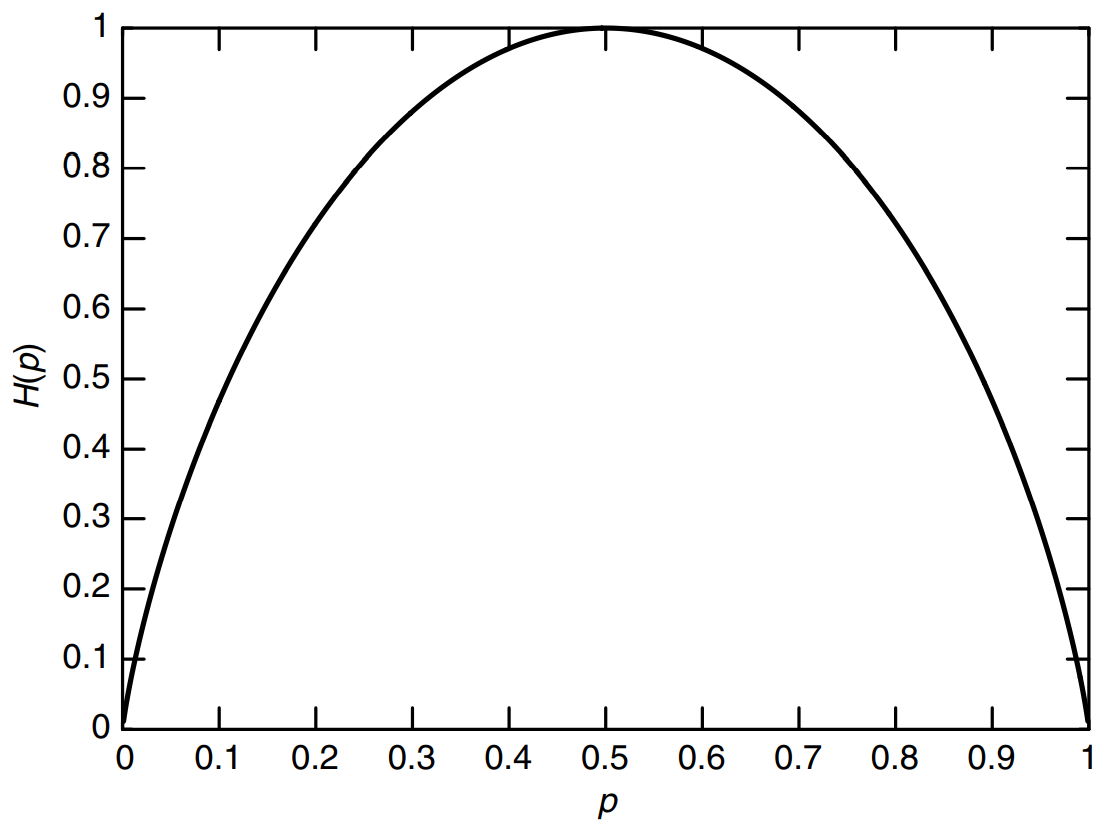
\includegraphics[width=0.4\linewidth]{screenshot005}
		\caption{$H(p)$ vs $p$ (originates from ``Elements of Information Theory", page 16)}
		\label{fig:EntropyvsP}
	\end{figure}
	
	
	
	%[book: p16: note should rename figure to axes to ” H(x) vs …”]
	Figure \ref{fig:EntropyvsP} displays when entropy reaches its maximum for the case of a random variable with 2 outcomes. We can see that the entropy, and thus, the information is largest when the probability of the two outcomes is equal to each other, namely $p(x_1)=p(x_2)=0.5$. Note that for a random variable $X$ with more than two events, $H(X)$ can be larger than one.
	
	\subsection{Kullback Leibler Divergence and Mutual Information} \label{cha:rel_entrop}
	The Kullback Leibler (KL) divergence, is defined in equation \ref{eq:kl}, where $p(\cdot)$ and $q(\cdot)$ denote probability density functions over the same sample space $\mathcal{X}$ \citep{coverElementsInformationTheory2006}. The KL divergence quantifies the ``dissimilarity" or ``divergence" between the two distributions. Note that $\kl{p(\cdot)}{q(\cdot)}$ does not necessarily equal $\kl{q(\cdot)}{p(\cdot)}$ and thus the metric is not symmetrical.
	
	\begin{equation}
		\kl{p(\cdot)}{q(\cdot)} = \sum_{x\in\mathcal{X}}p(x) \log \frac{p(x)}{q(x)} \label{eq:kl}
	\end{equation}
	
	
	
	% was rephrased by chat gpt
	The mutual information (MI) between two random variables $X$ and $Y$ can be computed as the KL divergence between their joint probability distribution, $p_{X,Y}(x,y)$, and the product of their marginal probability distributions, $p_X(x)$ and $p_Y(y)$ \citep{coverElementsInformationTheory2006}. The equation for mutual information then becomes:
	
	\begin{equation}
		I(X; Y) =  \kl{p_{X, Y}(x, y)}{p_X(x) p_Y(y)}
	\end{equation}
	
	As described by Cover and Thomas in their book ``Elements of Information Theory" \citep{coverElementsInformationTheory2006}, MI quantifies the amount of information $Y$ describes about $X$. An alternative definition is illustrated in \ref{eq:MI_reduce}. The equation provides us with an intuitive meaning for MI, corresponding to the surprise caused by $X$, which is reduced by the knowledge of $Y$. 
	\begin{equation}
		I(X;Y)= H(X) - H(X|Y) \label{eq:MI_reduce}
	\end{equation}
	In sections \ref{cha:bg_reconstr} and \ref{cha:bg_nce}, we discuss how these concepts from information theory are applied in representation learning.
		
		
		
		
		
		
		
		


\section{Representation Learning through Reconstruction Error} \label{cha:bg_reconstr}



% while supervised learning learning finds f given x -> y. performance gains may be obtained by manually transformating T(x) = z s.t f(z) = y. Self supervised representation learning attempts to automate the process of finding T.

%[what is repr learning]
One of the challenges in supervised learning is the constant need of large amounts of labelled data $\Dtrain = \{ \left( \vect{x}^{(1)}, \vect{y}^{(1)} \right), \left( \vect{x}^{(2)}, \vect{y}^{(2)} \right), \dots \}$. When this set is scarce, or the task becomes too complex to ensure good generalisation, transforming the feature space $\X$ into a lower-dimensional space $\Z$ can be a good solution to aid with learning for the downstream task $\f$. Meanwhile, an abundant amount of unlabelled data may already exist. Hence, when a labelled dataset is small, we would like to leverage a larger unlabelled dataset as a basis for learning.

In this section we investigate two self-supervised learning paradigms which learn the following transformation function solely from a feature space $\X$ and thus do not require any labels:
$$T: \X \rightarrow \Z$$
The simplified representations obtained from $\T$ can then serve as the input for a downstream task as follows:
\begin{align*}
	T(\vect{x}) &=  \vect{z} \\
	f(\vect{z}) &= \vect{y} 
\end{align*}
This process of learning a mapping function $\T$ which translates a feature vector $\vect{x}$ to a lower-dimensional representation $\vect{z}$ is commonly referred to as representation learning \citep{le-khacContrastiveRepresentationLearning2020}. 

In the following two subsections, we discuss two paradigms of representation learning with ANNs. The first paradigm learns representations by minimising a reconstruction error. The second learns its representations by contrasting them against noise. These two paradigms will lay the basis for our own contributions in chapter three.

\subsection{Autoencoders}
The encoding problem, introduced by Ackley and Hinton in 1985 \citep{ackleyLearningAlgorithmBoltzmann1985}, and later referred to as the autoencoder by Rumelhart et al. in 1986 \citep{rumelhartLearningInternalRepresentations1988}, considers the problem of learning compressed representations through neural networks \citep{rumelhartLearningInternalRepresentations1988, bankAutoencoders2021}. This is achieved through an ANN architecture consisting of two functions, an \textit{encoder} $E(\vect{x}) = \vect{z}$ and a \textit{decoder} $D(\vect{z}) = \vect{\tilde{x}}$.
%The first block is the encoder $E$ and receives input data which it encodes into a lower dimensional representation. The second block, called the decoder $D$, receives as input the latent representation and is tasked to reconstruct the original input. 
The lower-dimensional \textit{encoding} $\z$ obtained from $E(\x)$ will then serve as representation for downstream task $\f$.
The functions $\E$ and $D(\cdot)$ are simultaneously optimised by minimising the reconstruction error shown in the following equation:
\begin{equation}
	\mathcal{L} = \sum_{i = 1}^N l(\vecti{x}, \vecti{\tilde{x}})
\end{equation}
where $l$ refers to the error for a single data point, for instance, the $L^2$-norm, and $N$ the number data points. The dimension of $\vect{z}$ is typically smaller than the original dimension of $\vect{x}$. This results in the encoder having to define encodings that are as ``informative" as possible to reconstruct the original data \citep{bankAutoencoders2021}.

An example autoencoder architecture is depicted in figure \ref{fig:autoencoder}. Since an autoencoder is in fact a single ANN and $\z$ corresponds to the output produced by an intermediate hidden layer, $\z$ is also commonly referred to as a \textit{latent} representation. The space of all latent representations $\Z$ is known as the \textit{latent} space.
	\begin{figure}
		\centering
		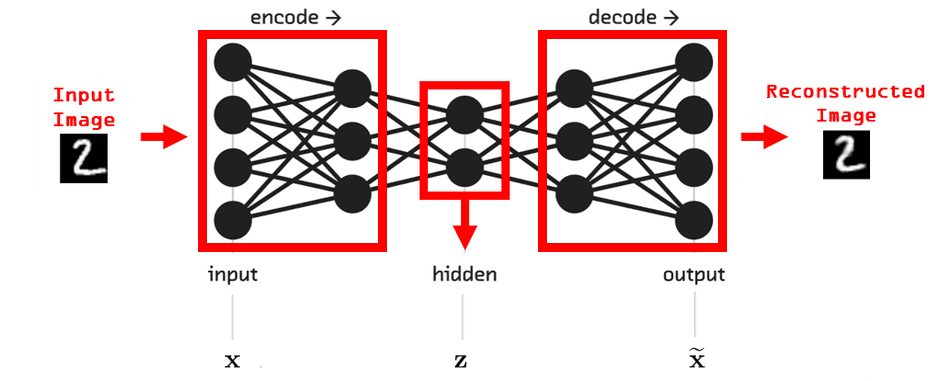
\includegraphics[width=0.7\linewidth]{autoencoder}
		\caption{Autoencoder architecture, adapted from \citep{karagiannakosHowGenerateImages2018}.}
		\label{fig:autoencoder}
	\end{figure}
While capable of learning compressed representations, autoencoders do not pose any restrictions on the latent space $\Z$. As a result, the representations may be meaningful to computers, but non-interpretable to humans. For instance, given the left image depicted in figure \ref{fig:latent_space_2d} which depicts an autoencoder's two-dimensional latent space, it is almost impossible to infer in advance what the corresponding digit would be when interpolating a new $\z$ somewhere in between the encodings corresponding to digit 0 (red) and 1 (blue). In addition, slight changes to $\z$ may result in significant changes to its decoded counterpart $\x$. Finally, attempting to understand an autoencoder's latent space $\Z$ becomes even more infeasible as the dimension of $\Z$ increases.

\begin{figure}
	\centering
	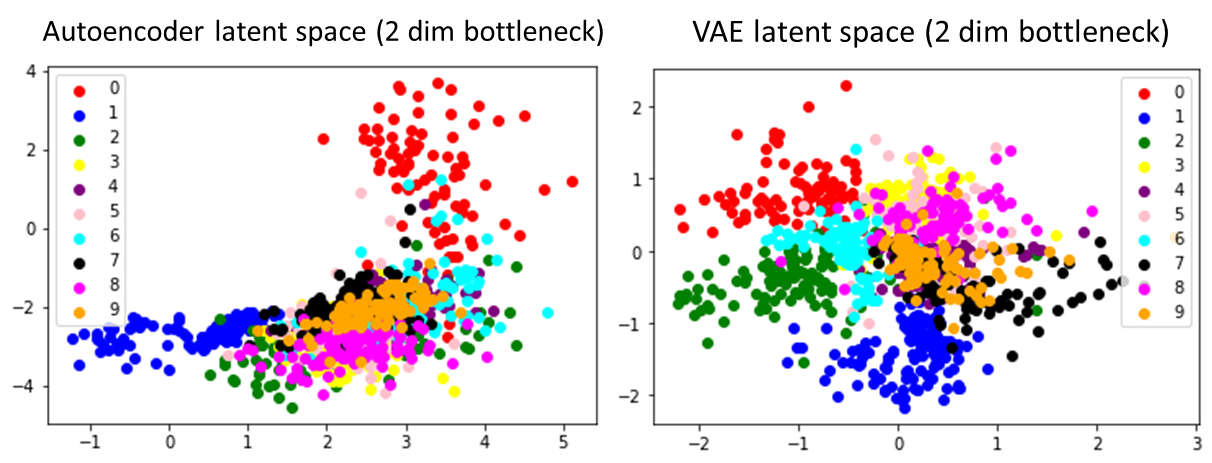
\includegraphics[width=0.7\linewidth]{screenshot021}
	\caption{ Latent space of autoencoder (left) and VAE (right), learned from the MNIST dataset, a dataset consisting of images of handwritten digits between 0 and 9 \citep{lecunGradientbasedLearningApplied1998}. The ANNs have not received any explicit information of the labels of the dataset. 
	%The VAE's latent space, depicted in the right image, is optimised to be standard normally distributed. The latent vectors $\vect{z}$ are distributed according to the two-dimensional normal distribution $\sample{\vect{z}}{\standardnormal}$, where $\bm{\mu}$ is the two-dimensional zero vector. $\identitymtx$ is the $2 \times 2$ covariance matrix with ones on the diagonal and zeroes elsewhere.
}
	\label{fig:latent_space_2d}
\end{figure}



\subsection{Variational autoencoders} \label{cha:bg_vae}
% notes: 
%1) discuss why, (latent space gaussian)
%2) architecture predicting values
%3) explicit elbo (where q is optimised to be Gaussian) and give intuitions how it squishes all data points together
%4) can be used for latent space, or also 
%4) link with maximising likelihood -> p(x) and how minimises kl divergence between approx and kl divergence

Similar to traditional autoencoders, variational autoencoders (VAE) learn representations that contain the important information necessary to reconstruct the data. VAEs maintain the same structure as autoencoders, consisting of an encoder $E(\vect{x}) = \vect{z}$ and decoder $D(\vect{z}) = \vect{\tilde{x}}$. However, an additional constraint is applied to the latent space $\Z$ \citep{doerschTutorialVariationalAutoencoders2021, davidfosterVariationalAutoencoders2023, kingmaAutoEncodingVariationalBayes2022, kingmaIntroductionVariationalAutoencoders2019, cinelliVariationalMethodsMachine2021}. The latent representations $E(\vect{x}) = \vect{z}$ are samples from multivariate distributions, which we will denote by 

$$\sample{\vect{z}}{\qvae} \quad \text{or equivalently: } \quad \sample{\vect{z}}{\qvaeBlank}$$

Thus, given a feature vector $\x$, we obtain its corresponding \textit{encoding} or \textit{latent representation} $\z$ by taking a sample from a distribution. This distribution is commonly known as the \textit{posterior} distribution, we will define it in more detail in a following paragraph. The encoder function $\E$ in VAEs is thus nondeterministic and computing $E(\vect{x}) = \vect{z}$ twice may result in two different $\z$s both corresponding to the same $\x$. In a following paragraph, we will discuss how to achieve this nondeterministic behaviour using ANNs.

By defining the latent representations as samples from distributions, we can pose the same constraints on the quality of the representations $\z \in \Z$ as in traditional autoencoders, but also additional constraints on how the latent space $\Z$ is organised. The additional constraints posed by VAEs on $\Z$ will result in a more interpretable space, where $\z$'s underlying components can be better understood. This will be achieved by enforcing each distribution $\qvaeEmptyZandXI$ corresponding to a particular $\vecti{x}$, to be ``similar" to a chosen \textit{prior} distribution $p(\z)$. Typically, the prior $p(\z)$ is set to the standard normal distribution $\standardnormal$ \citep{davidfosterVariationalAutoencoders2023}. The result of this setup can be observed in the latent space depicted in the right plot of figure \ref{fig:latent_space_2d} where all $\z$s are attracted to the origin.

In the following subsections, we will explore VAEs in more detail. We begin with a discussion on the process of imposing constraints on $\Z$, which leads to the VAE loss function. Next, we investigate how ANNs can be utilised to simulate sampling from distributions. Finally, we examine how VAEs enable the creation of interpretable representations and how they can be used to generate novel data.




\subsubsection{The loss function}	
% def q

	So far, we have learned that Variational Autoencoders (VAEs) use an encoder $E(\x) = \z$ to create a latent representation $\z$ of the input feature vector $\x$, where $\z$ is a sample from the distribution $\sample{\z}{\qvae}$. %Equivalently, for each $\x$, there exists a unique distribution $q(\z)$ that characterizes $\qvae$ \citep{volodymyrkuleshovVariationalAutoencoder2023}. 
	We can then define $\qvae$ as a Gaussian with independent components, parametrised by $\mufat$ and covariance matrix $\diagsigma$. We obtain the following definition:
	\begin{equation}
		\qvae = \normalNoI \label{eq:definition_q}
	\end{equation}
	where $\diagsigma$ denotes the covariance matrix with $\sigmafat$ on the diagonal and zeroes elsewhere. It is important to recognise that $\mufat$ and $\sigmafat$ are different for every $\x$. The two parameters will be computed by an ANN.


% loss
	The representations are optimised to minimise two measurements: one, the reconstruction error, and secondly, the dissimilarity from the latent distributions to a chosen prior $p(\z)$. %$\standardnormal$.
	The loss function to be optimised for a single data point $\vecti{x}$ is shown in the equation below.
	\begin{equation}
		\mathcal{L} (\vecti{x}) = \elboexplicit \label{eq:elbo_explicit_intial}
		%\mathcal{L}_{\theta, \phi} (\vecti{x}) = \elboexplicit \label{eq:elbo_explicit_intial}
	\end{equation} % src: ref to slides ugent
	Here, $p(\cdot)$ refers to the prior distribution, which is different from $\pthetaxzi$.
	% 1) reconstruction error
	Although $\mathcal{L}$ may seem daunting at first, we will decompose its components. The loss function is made up of two terms, the left term corresponds to the reconstruction error, while the second term poses constraints on the latent space. Let us focus on the reconstruction term first.
	
	\begin{equation}
		\reconstr \label{eq:reconstr}	
	\end{equation}

	In a traditional autoencoder we optimise $D(E(\vecti{x})) = \vecti{\tilde{x}}$ such that $\vecti{x} \approx \vecti{\tilde{x}}$. We will now show that the reconstruction term in equation \ref{eq:reconstr} achieves a similar goal for VAEs. Here, $\pthetaxzi$ is a distribution over $\vecti{z}$ where $\vecti{x}$ is fixed, and the latent representation $\vecti{z} = E(\vecti{x})$ is sampled from the Gaussian distribution $\sample{\vecti{z}}{\qphizxblank}$. The objective is to ensure that $D(\vecti{z}) \approx \vecti{x}$. However, since $\vecti{z}$ is sampled from a Gaussian distribution, the $\vecti{z}$'s close to the mean $\mui$ are more likely to be sampled than those further away. Thus, for these $\vecti{z}$'s, we'd like the probability of corresponding to the actual $\vecti{x}$ to be high, or equivalently we want $\pthetaxzi \approx 1$ \citep{cinelliVariationalMethodsMachine2021}. Finally, by adding a negative sign in front, maximising this probability is equivalent to minimising the negative probability. In practice, this term is approximated through mini-batches with the mean squared error. %todo: look into max like estim, as there hopefully i can find a meaningful defintion for "maximising..."
	

% 2) latent space
	Optimising the second term of equation \ref{eq:elbo_explicit_intial} poses the constraints on the distributions $\qphizxblank$. 
	\begin{equation}
		%\latentspaceconstraintstandardgaussian
		\latentspaceconstraint \label{eq:latent_space_constraint}		
	\end{equation}
	Again, this metric should be minimised. As we discussed in chapter \ref{cha:rel_entrop}, KL divergence can be considered as a dissimilarity measure between two distributions. Hence, this value is small when the two distributions are similar. The prior distribution $\pzblank$ is a fixed distribution which is chosen by the user, typically defined as $\standardnormal$. Minimising this metric will result in moving each distribution $\qphizx$, corresponding to a value $\vecti{x}$, close to $\standardnormal$. This idea is depicted in figure \ref{fig:twogaussiandistributions}. When $\pzblank = \standardnormal$, equation \ref{eq:latent_space_constraint} becomes:
	$$\latentspaceconstraintstandardgaussian$$
	
	\begin{figure}
		\centering
		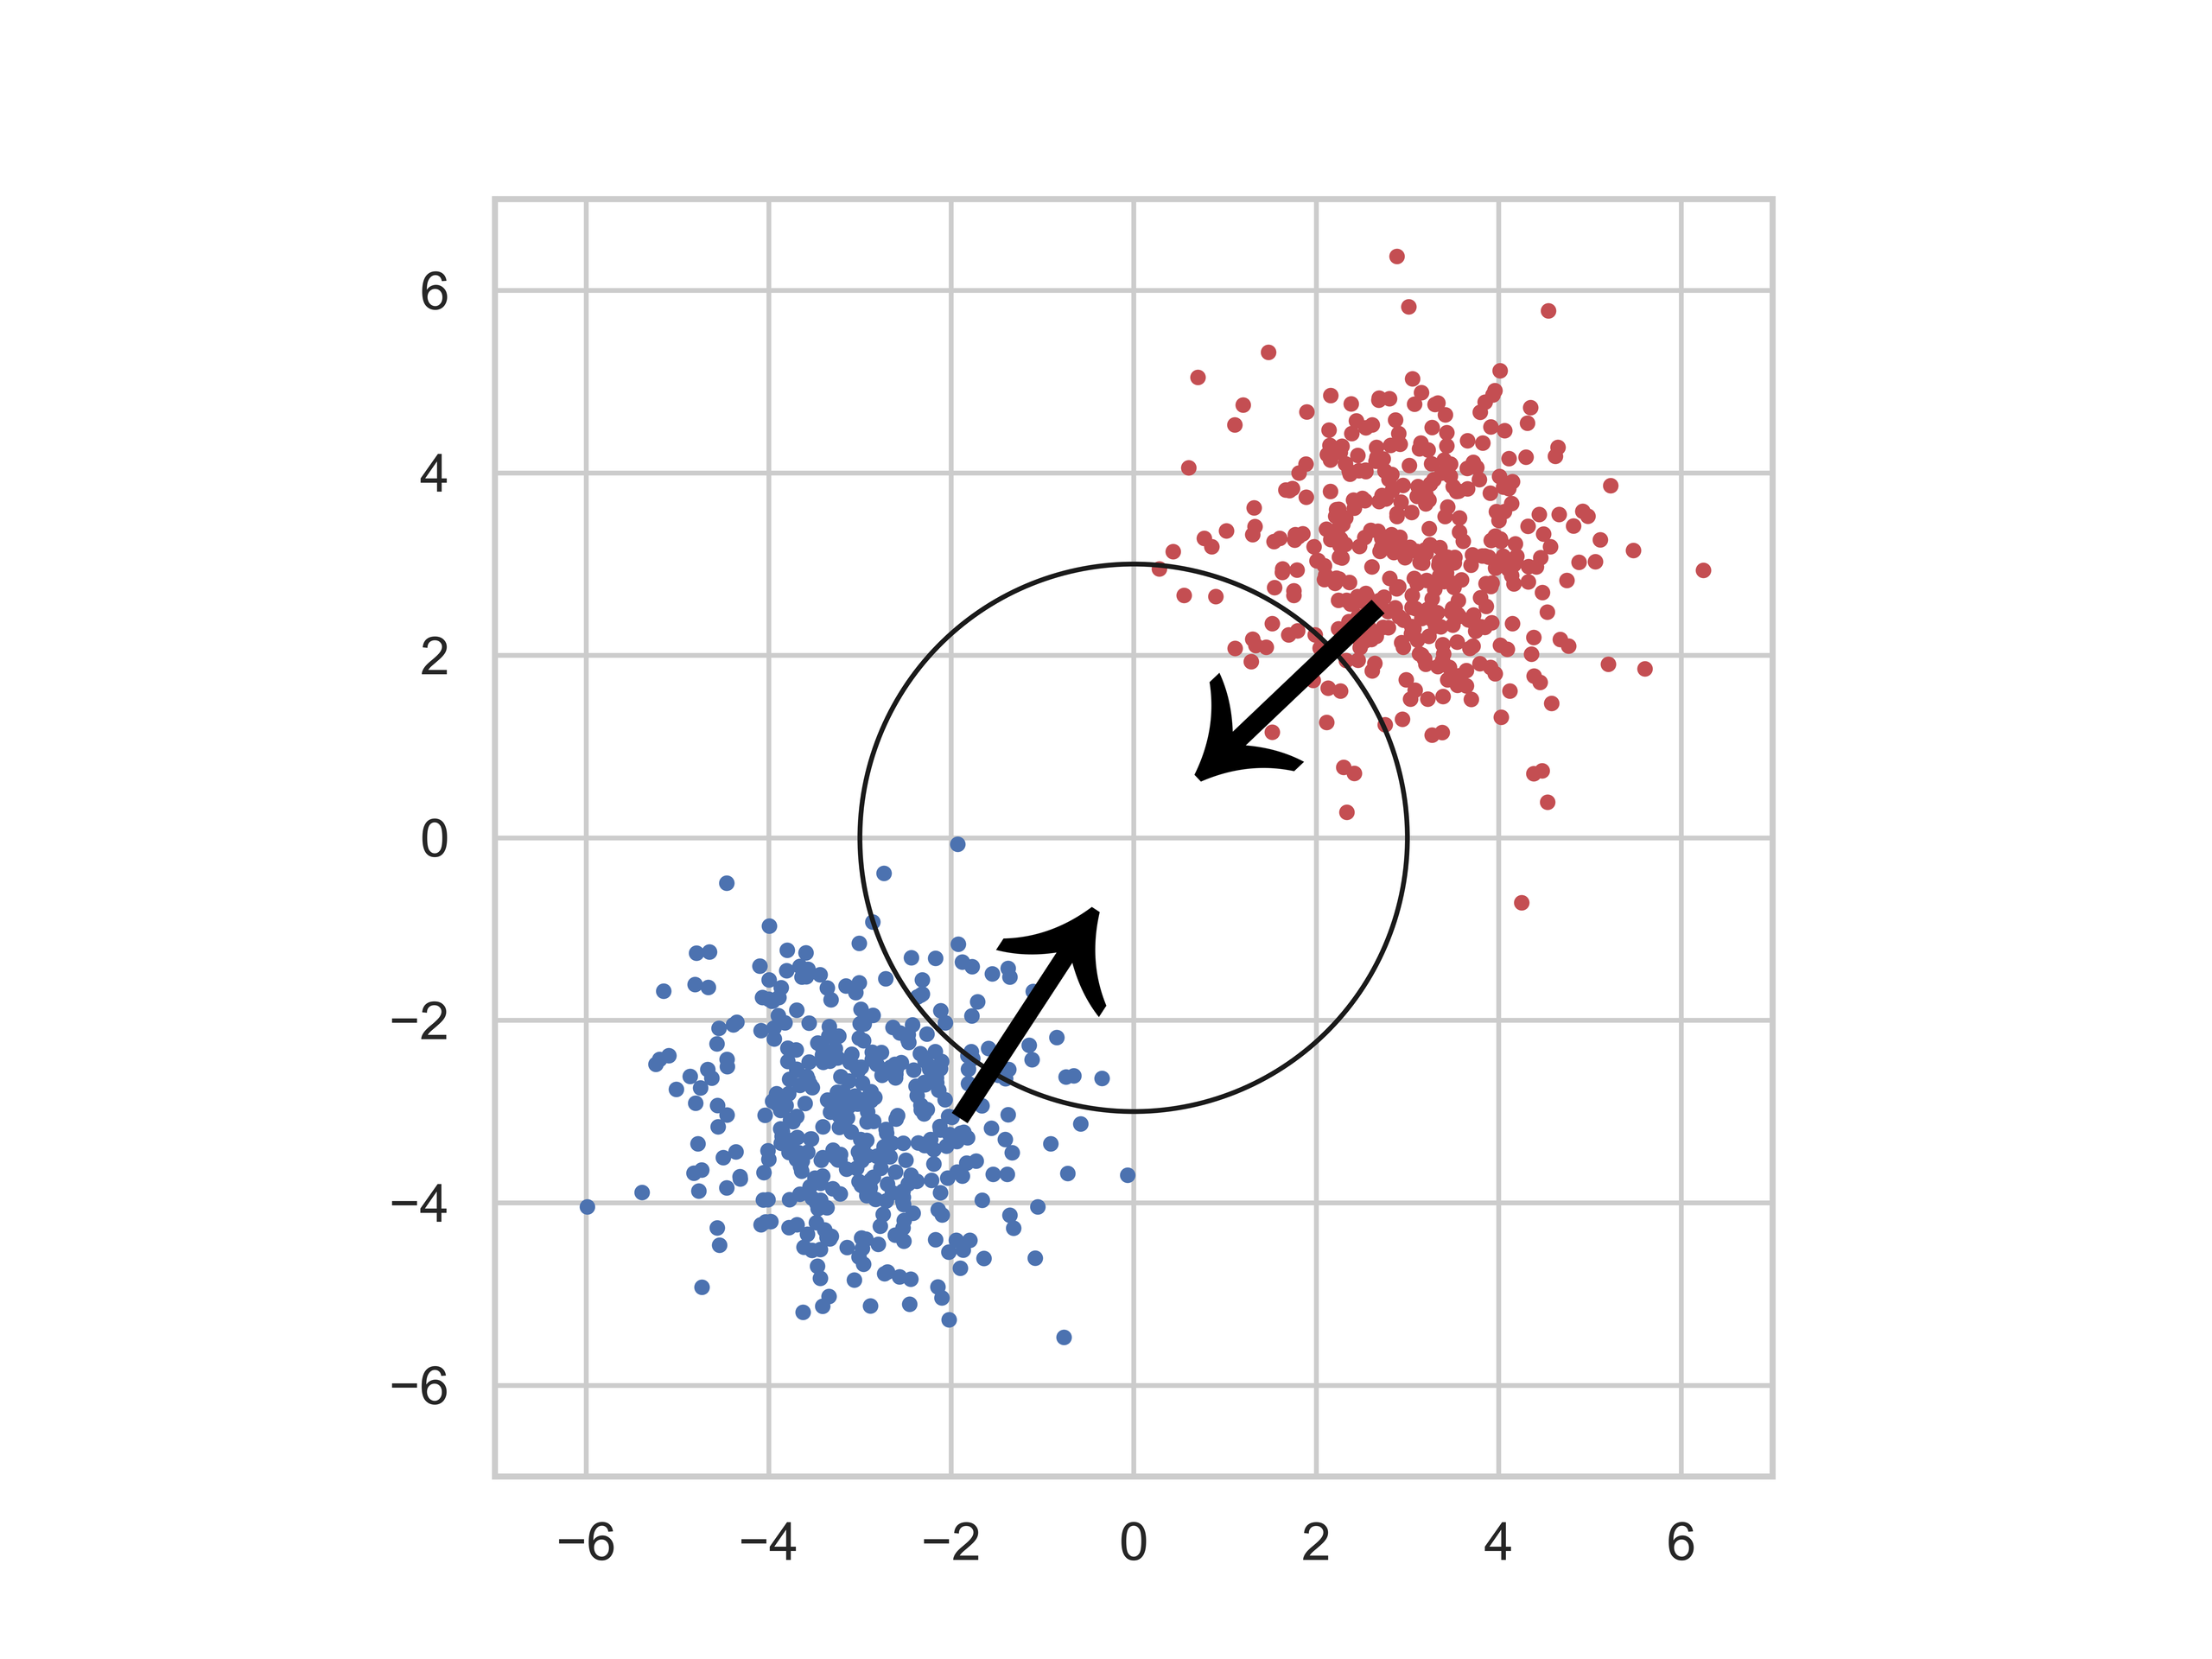
\includegraphics[width=0.7\linewidth]{two_gaussian_distributions}
		\caption{200 samples $\vecti{z}$ and $\vectj{z}$ from feature vectors $\vecti{x}$ and $\vectj{x}$, respectively, represented by red and blue data points. The prior $p(\vect{z})$ is set to the standard normal, and the regularisation term of VAE's loss pushes the latent space towards the origin.}
		\label{fig:twogaussiandistributions}
	\end{figure}
	When $\qphizxblank = \normal$, one can algebraically prove, that optimising the above equation is equivalent to optimising the following \citep{kingmaAutoEncodingVariationalBayes2022}: 
	\begin{equation}	
		\kl{\normal}{\standardnormal} = \latentspaceconstraintclosedform
	\end{equation}
	where $\sigma_k^{(i)}$ and $\mu_k^{(i)}$ correspond to the components of the predicted vectors $\sigmai$ and $\mui$, respectively. The latent space has dimensionality $D$.
	



%\textbf{How: predict distributions}

\subsubsection{Simulating distributions through neural networks}
	Computing $E(\xith)$ results in an encoding $\zith$ which is sampled from $\sample{\zith}{\qvaeEmptyZandXI}$. We will now discuss how ANNs can emulate the stochastic behaviour of sampling from a distribution. As discussed in equation \ref{eq:definition_q}, distribution $\qvaeEmptyZandXI$ is parametrised as a factorised Gaussian with mean $\mui$ and covariance matrix $\diagsigmai$. The entire distribution can thus be modelled by an ANN which takes as input $\xith$ and generates the two corresponding vectors $\mui$ and $\sigmai$. Finally, a sample $\vecti{z}$ can be obtained as follows:
	\begin{equation}
		\vecti{z} = \mui + \sigmai \odot \epiloni
	\end{equation}
	where $\epiloni$ corresponds to a sampled value $\samplestandardnormal{\epiloni}$ and $\odot$ is element-wise multiplication. Computing $\vecti{z}$ through $\epiloni$, rather than directly sampling from $\sample{\vecti{z}}{\normal}$ is referred to as the parametrisation trick and allows for gradients to freely backpropagate through the layer \citep{davidfosterVariationalAutoencoders2023}. The decoder $D(\zith) = \vecti{\tilde{x}}$ can remain identical to the traditional autoencoder's decoder. An overview is presented in figure \ref{fig:vae-repr}.
	
	\begin{figure}[h]
	\centering
	\tikzstyle{arrow} = [thick,->,>=stealth]
	\begin{tikzpicture}[
		AnnNode/.style={trapezium, draw=black,
			trapezium stretches=true,
			minimum width=2cm, 
			minimum height=1.5cm,
			rotate=-90,
			trapezium angle=75,
			very thick},
		]
		
		\node[AnnNode] (enc) {\rotatebox{90}{$E(\xith)$}};
		\node[AnnNode] (dec) [right of=enc, xshift=1.5cm] {\rotatebox{90}{$D(\zith)$}};
		
		% enc edges
		\draw[->] ++(-2.5, 0) -- (enc.south) node[above, midway] {$\xith \in \D$};
		\draw[->] 
		[transform canvas={yshift=.7em}] 
		(enc.north) -- ++(1.5, 0) node[above, midway] {$\mui$};
		\draw[->] 
		[transform canvas={yshift=-.7em}] 
		(enc.north) --  ++(1.5, 0) node[below, midway] {$\sigmai$};
		
		\node 
		[transform canvas={xshift=5.5em}] 
		(bracket1) at (enc.north) {\Huge \} };
		
		\node 
		[transform canvas={xshift=10em}] 
		(sample z) at (enc.north) {$\sample{\zith}{\qvaeEmptyZandXI}$ };
		
		
		
		% dec edges
		\draw[->] ++(-2.5, -2.5) -- (dec.south) node[above, midway] {$\zith$};
		\draw[->] 
		(dec.north) -- ++(1.5, 0) node[above, midway] {$\vecti{\tilde{x}}$};	  		
		
		
		
	\end{tikzpicture}
	\caption{High level view of a VAE.}
	\label{fig:vae-repr}
\end{figure}





% from img
% Both blocks depict a neural network. The upper block is the encoder and the lower block the decoder. The upper block receives a data points $\vect{x}$ and produces the parameters of $\qphizx$. Since we choose to model $\qphizx$ as a Gaussian with independent components, the covariance matrix $\covariancemtx$ is zero everywhere except for the diagonal. This way the diagonal values, representing the standard deviations, can be represented via a single vector $\sigmai$. The vectors $\mui$ and $\sigmai$ are $\mu(\vecti{x})$ and $\sigma(\vecti{x})$, respectively. These are the output of the encoder block and form the parameters for $\qphizx$. A single neural network with parameter weights $\phi$ is used to simulate $\qphizx$ for every $\vecti{x} \in \mathcal{D} $. This strategy of sharing $\phi$ across data points is refered to as "amortised variational inference" \cite{kingmaIntroductionVariationalAutoencoders2019}.
	
	
	
	




	
	


\subsubsection{Generating new data and interpretability}	
	Due to the VAE's regularisation term, all encodings are pushed towards the centre as depicted in figure \ref{fig:twogaussiandistributions}. Additionally, the space of encodings corresponding to a single $\xith$ is an entire neighbourhood around a particular $\mufat$ and $\sigmafat$. These two properties ensure a well-covered and uninterrupted space around the origin with smooth transitions on the generative factors between latent representations \citep{davidfosterVariationalAutoencoders2023}. As a result, new samples from the dataset can be generated by discarding the VAE's encoder and providing standard normal noise to the decoder instead. It is important to understand that this method only works for VAEs and not for the traditional autoencoder. This is because autoencoders do not pose any additional constraints on the latent space. Generating new data points from random noise via a traditional autoencoder may result in nonsense generations as the random noise may be too different from the latent space it was trained on. As a result, there are no guarantees that the autoencoder's decoder will generalise to these random representations.
	
	Additionally, for the same reason, we can interpolate between encodings obtained from the data. The interpolated encoding can then decoded to the original space. We can observe the specific information contained in each of the representations' features through the decoder, resulting in a significant improvement in interpretability.
	% TODO: if time permits, this sectino could be written better ^^ ik zou met ven diagrammen kunnen werken.
	
	% TODO: maybe check if everything is present and argumentation is okay.	
	%	o reiley:
		%Firstly, we now have a well-defined distribution that we can use for choosing points in the latent space—the standard normal distribution. Secondly, since this term tries to force all encoded distributions toward the standard normal distribution, there is less chance that large gaps will form between point clusters. Instead, the encoder will try to use the space around the origin symmetrically and efficiently.
		
		
		%\textit{Previously, we saw how there was no requirement for the latent space to be continuous—even if the point (–2, 2) decodes to a well-formed image of a sandal, there was no requirement for (–2.1, 2.1) to look similar. Now, since we are sampling a random point from an area around $z_mean$, the decoder must ensure that all points in the same neighbourhood produce very similar images when decoded so that the reconstruction loss remains small. This is a very nice property that ensures that even when we choose a point in the latent space that has never been seen by the decoder, it is likely to decode to an image that is well-formed.} - o reiliy
		%
		
	
	
	
	
	
	
	
	
	



%\subsubsection{[TODO] Relation with variational inference / derivation of ELBO loss}
%	
%	%A mapping function $f_W(x) = y$ can be predict distributions by predicting the parameters of the the distribution (mu, sigma for Gaussian distributions).
%	%
%	%Rather than directly learning parameters $\phi$ that map a data point $\vecti{x}$ to latent distribution $p(\vect{z} \mid \mathbf{x}^{(i)})$, an \textit{approximate distribution} $\qzx$ is learned that approximates $p(\vect{z} \mid \vecti{x})$. Through gradient descent parameters for $\phi$ can be achieved, by minimising the KL divergence between the two distributions. $\condq{\vect{z}}{\vecti{x}}$ will is expressed as Gaussian distribution.
%	%
%	%
%	%\begin{equation}
%	%	\kl{\qprobzx}{\probzx} \label{eq:kl_q_p}
%	%\end{equation}
%	%
%	%Yet, the idea is nice, optimising $\qprobzx$ to approximate $\probzx$ sounds nice, it is only possible when $\probzx$ is known, which it is not. If it was, there was no need to approximate it.
%	%
%	%Equation \ref{eq:kl_q_p} is thus intractable to compute, yet the following is true:
%	%
%	%\begin{equation}
%	%	\begin{aligned}
%	%		\kl{\qprobzx}{\probzx} & = \expectedsamplezq \left[ \log \frac{\qzx}{\pzx} \right] \\
%	%		& = ... (todo) \\
%	%		& = - \left( \elbo \right) + \logevidence
%	%	\end{aligned}
%	%\end{equation}
%	%
%	%By replacing the terms, we obtain the following equation:
%	%
%	%\begin{equation}
%	%	\begin{aligned}
%	%		\logevidence & = 
%	%		\klapproxposterior + \elbo \\
%	%		& = \klapproxposterior  + \lelbo
%	%	\end{aligned}
%	%\end{equation}
%	%
%	%We can observe that the KL divergence between the true and approximate posteriors, $p$ and $q$ respectively, is bounded by $\logevidence$. Hence, although $\pzx$ is unknown, maximising $\lelbo$ results in minimising the KL divergence. Also notice that $\kl{\qprobzx}{\probzx} >= 0$, and thus the maximum value for $\lelbo$ results in a KL divergence between the posteriors of zero. It thus suffices to maximise $\lelbo$, or equivalently minimise $-\lelbo$. The loss for a single data point $\vecti{x}$ then becomes
%	
%	%TODO \textbf{todo: in paper variational bayes, they refer to p(x) as p theta, but in slides ugent not?}. \textbf{todo: why cant p(x) be very big then? probably has something to do with jensens inequality.}
%	
%	
%	
%	
%	\begin{equation}
%		\begin{aligned}
%			- \lelbo & = - \elbo \\  
%			& = \elboexplicit \label{eq:elboexplicit} \\
%		\end{aligned}	
%	\end{equation} % src: ref to slides ugent
%	
%	Where the first term is reconstruction error and second is regularisation. Hence minimising the KL divergence between the two posteriors is equivalent to minimising the divergence between the approximate posterior $\qzx$ and the \textbf{marginal or prior?} $\pz$.
%	
%	$p(z)$ in the equation is usually chosen to be the standard normal distribution $\mathcal{N}(0, I)$, such that a closed form solution exists. As such, when $p(z)$ corresponds to the standard normal, and $\qzx$ is a multidimensional Gaussian with mean vector $\mui$ and covariance matrix with independent dimensions, such that the diagonal corresponds of a vector standard devisations $\sigmai$, then the KL divergence has the following closed form:
%	
%	\begin{equation}	
%		\kl{\normal}{\standardnormal} = \latentspaceconstraintclosedform
%	\end{equation}
%	
%	For the equation above, gradients can easily be back propagated through machine learning libraries such as Tensor Flow. We still require a method for computing the gradient of the first term in $\lelbo$. % todo: gradient van linker kan door sampling en mini batch.
%	
%	
%	
%	
	
	
	
	
	
	
	
	%Recent Advances in Autoencoder-Based:
	%Representation Learning https://arxiv.org/pdf/1812.05069.pdf
	%they speak about disentanglement of vae and indepndent features
	
	%Understanding disentangling in β-VAE
	%https://arxiv.org/pdf/1804.03599.pdf
	%"β-VAE aligns latent dimensions with components that make different contributions to reconstruction"
	%Our key hypothesis is that β-VAE finds latent components which make different contributions to the log-likelihood term of the cost function (Eq. 5). These latent components tend to correspond to features in the data that are intuitively qualitatively different, and therefore may align with the generative factors in the data.
	
	
	
	
	
	
	
	
	
	
	
	%- \subsubsection{reparametrisation trick}
	%o reiley:
	%\textit{THE REPARAMETERIZATION TRICK
	%	Rather than sample directly from a normal distribution with parameters $z_mean$ and $z_log_var$, we instead sample epsilon from a standard normal and then manually adjust the sample to have the correct mean and variance.}
	%\textit{This is known as the reparameterization trick and is important as it means gradients can backpropagate freely through the layer. By keeping all of the randomness of the layer contained within the variable epsilon, the partial derivative of the layer output with respect to its input can be shown to be deterministic (i.e. independent of the random epsilon), which is essential for backpropagation through the layer to be possible.}
	
	%\subsubsection{the loss function - from oreiley}
	%The Loss Function
	%Previously, our loss function only consisted of the reconstruction loss between images and their attempted copy after being passed through the encoder and decoder. The reconstruction loss also appears in a variational autoencoder, but we require one extra component: the Kullback–Leibler (KL) divergence term.
	%
	%KL divergence is a way of measuring how much one probability distribution differs from another. In a VAE, we want to measure how much our normal distribution with parameters z_mean and z_log_var differs from a standard normal distribution. In this special case, it can be shown that the KL divergence has the following closed form:
	%
	%kl_loss = -0.5 * sum(1 + z_log_var - z_mean ^ 2 - exp(z_log_var))
	%or in mathematical notation:
	%
	%The sum is taken over all the dimensions in the latent space. kl_loss is minimized to 0 when z_mean = 0 and z_log_var = 0 for all dimensions. As these two terms start to differ from 0, kl_loss increases.
	%
	%In summary, the KL divergence term penalizes the network for encoding observations to z_mean and z_log_var variables that differ significantly from the parameters of a standard normal distribution, namely z_mean = 0 and z_log_var = 0.
	%
	%Why does this addition to the loss function help?
	%
	%Firstly, we now have a well-defined distribution that we can use for choosing points in the latent space—the standard normal distribution. Secondly, since this term tries to force all encoded distributions toward the standard normal distribution, there is less chance that large gaps will form between point clusters. Instead, the encoder will try to use the space around the origin symmetrically and efficiently.
	%
	%In the original VAE paper, the loss function for a VAE was simply the addition of the reconstruction loss and the KL divergence loss term. A variant on this (the 
	%-VAE) includes a factor that weights the KL divergence to ensure that it is well balanced with the reconstruction loss. If we weight the reconstruction loss too heavily, the KL loss will not have the desired regulatory effect and we will see the same problems that we experienced with the plain autoencoder. If the KL divergence term is weighted too heavily, the KL divergence loss will dominate and the reconstructed images will be poor. This weighting term is one of the parameters to tune when you’re training your VAE.
	


\subsubsection{Disentanglement of latent representations and posterior collapse} \label{cha:disentang}
	\cite{higginsBetaVAELearningBasic2022} extend the VAE framework through the introduction of a slight modification of the loss function, resulting in $\beta$-VAE. An additional hyper-parameter $\beta$ is introduced to the VAE's loss function which controls the weight of the regularisation term:
	$$
	\mathcal{L}_{\theta, \phi} (\vecti{x}) = \betaelboexplicit
	$$
	
	Setting the prior to a standard normal distribution ($p(\z) = \standardnormal$) encourages disentangled representations, where each variable is sensitive to a specific generative factor \citep{higginsBetaVAELearningBasic2022, bengioRepresentationLearningReview2013a}. For example, in an image of a face, altering one component of the representation would only change the smile, while other features like skin colour and brightness remain constant. Such disentangled representations are interpretable, making it easier to understand the underlying structure of the representation and what information each variable contains.
	
	However, a trade-off must be made between accuracy and disentanglement. A small $\beta$ value (close to 0) results in high a reconstruction accuracy but weak constraints on disentanglement, while a large $\beta$ value (above 1) puts large emphasises on disentanglement at the cost of accuracy. If $\beta$ becomes too large, the posteriors $\qphizx$ corresponding to each data point $\vecti{x}$ can become equal to the prior $p(\vect{z})$, resulting in no information contribution, which is known as posterior collapse \citep{lucasUnderstandingPosteriorCollapse2022}.
	

	
	
	
% TODO: explain about gaps, etc
% i said z's are closer to (0, 0). why do we care? -> similar points are still clustered together, however, there will not be any gaps in the latent space. can thus interpolate between latent representations to find meaningful datapoints.

%o reiley:
%\textit{"A multivariate standard normal distribution is a multivariate distribution with zero valued mean vector and identity covariance matrix."} - 
%%https://learning.oreilly.com/library/view/generative-deep-learning/9781098134174/ch03.html#normal_distribution
%
%\textit{Previously, we saw how there was no requirement for the latent space to be continuous—even if the point (–2, 2) decodes to a well-formed image of a sandal, there was no requirement for (–2.1, 2.1) to look similar. Now, since we are sampling a random point from an area around $z_mean$, the decoder must ensure that all points in the same neighbourhood produce very similar images when decoded, so that the reconstruction loss remains small. This is a very nice property that ensures that even when we choose a point in the latent space that has never been seen by the decoder, it is likely to decode to an image that is well formed.} - o reiliy
%
	
	
	
	
	
	
	
	
	
	
	



\section{Representation learning through Noise Contrastive Estimation} \label{cha:bg_nce}
In the following two sections, we discuss Contrastive Predictive Coding (CPC) and Greedy InfoMax (GIM). We will use GIM as the basis for our own experiment in the following chapter. However, GIM continues from the concepts introduced in CPC and a good understanding is needed to understand the contributions of GIM.


\subsection{Contrastive Predictive Coding}
	CPC is an unsupervised learning approach, again with the objective of learning (lower-dimensional) representations from high dimensional data \citep{oordRepresentationLearningContrastive2019}. While the objective is thus the same as for the autoencoders discussed in the previous section, CPC achieves its representations entirely differently. An autoencoder's objective is to define a compressed representation from which the original data can be recovered. However, when working with sequential data $\x_1,\x_2,~\dots, ~\xt,~\dots$, simply compressing patches $\x_i$ of the sequence without considering the relation with nearby patches can result in suboptimal encodings, as contextual information between patches is not encoded directly into the representation \citep{shah92LearningGood2020}.
	%ChatGPT generated: In contrast, CPC considers the relationship between patches of the sequence to capture contextual information, making it a better option for representing time-series data.


\begin{figure}[h] % cpc overview
	\centering
	\includegraphics[width=0.7\linewidth]{"cpc overview"}
	\caption{Overview of Contrastive Predictive Coding, originates from \citep{oordRepresentationLearningContrastive2019}.}
	\label{fig:cpc-overview}
\end{figure}

%\textbf{[maintain information between patches by predicting the future based on the past? + architec fig + var names]} \\
	% todo
	CPC deals with these context issues by maximising the shared information between the extracted representations of temporally nearby patches \citep{lowePuttingEndEndtoEnd2020a}. We will discuss this concept in more detail in this section. For now, we would like to draw the reader's attention to figure \ref{fig:cpc-overview}. The figure depicts a high-level view of how this idea is achieved by producing two latent representations $\vect{z}_i$ and $\vect{c}_i$. An audio sequence of undefined length is split up into patches $\x_1 \dots \x_n$ where each $\x_i$ is a vector of fixed length, containing for instance 10ms of speech audio. Each patch $\x_i$ is encoded into latent representation $\zt$, defined as follows:
	
	$$
	\zt = g_{enc}(\xt) .
	$$
	
	$g_{enc}( \cdot )$ is for instance a ConvNet. The latent representations $\z_1 \dots \z_n$ are obtained independently from each other and do not yet contain any contextual information. This is achieved through $g_{ar}( \cdot )$, an autoregressor, which encodes all previous $\z_1 \dots \zt$ into a single representation $\ct$:
	
	$$
	\ct = g_{ar}(\z_1 \dots \zt)
	$$
	
	Either $\zt$ or $\ct$ could be used as the latent representation for downstream tasks. \cite{oordRepresentationLearningContrastive2019} suggest using $\ct$ for tasks where context about the past is useful, for instance, speech recognition, and $\zt$ when the historic context is not useful. As shown in figure \ref{fig:cpc-overview}, the encodings from sequential data of undefined length, may correspond to a series of latent representations $\vect{c}_1, \vect{c}_2, \dots $ or $\z_1, \z_2, \dots $. In the case of downstream tasks which require a single representation vector, \citeauthor{oordRepresentationLearningContrastive2019} propose to pool the sequence of vector representations into a single vector.
	

\subsubsection{Slowly varying features}
%\textbf{[assume slow features. + why maxim mutual info? between past and future]}\\
	The temporally nearby patches $\z_{t+1}$ and $\ct$ are optimised to preserve shared information, while discarding differences. Before we discuss how to obtain such representations, we first motivate why defining representations in this fashion makes sense.
	
	Consider we would like to define useful representations for sequential data such as speech signals. Then it is not unlikely to believe that the conveyed information at time step $t$ and $t+k$ contains some redundancy, such as pitch, frequency, tone, etc. \citep{raoUnderstandingGradientIsolatedLearning2020}. Meanwhile, large changes of the signal in a small time window may be the result of noise. Sequential data which poses these slowly varying features are commonly referred to as ``slow-features" \citep{zhangSlowFeatureAnalysis2012}. CPC leverages these slowly varying features, by encoding the underlying shared information between different patches while at the same time discarding low-level information and noise that is more local \citep{oordRepresentationLearningContrastive2019}.


\subsubsection{The loss function}
%\textbf{[discriminate pos from neg samples + formal MI]}\\
	% the latent representations are optimised through a similarity function f. It will turn on that optimising the similarity between two representations is equivalent to maximising their mutual information.
	
	
	CPC learns preserve information between temporally nearby representations, by solving another task. In particular, CPC learns to discriminate subsequent \textit{positive} samples $\ztk$ from \textit{negative} random samples $\zj$. This is achieved through a similarity function $f_k(\cdot)$, which scores the similarity between two latent representations \citep{lowePuttingEndEndtoEnd2020a}. It is defined as a log bilinear model as follows:
	\begin{equation} % f_k
		\fkdefinition \label{eq:fk}
	\end{equation}
	where $W_k$ is a weight matrix which is learned. $f_k( \zj , \ct )$ thus quantifies how likely the context $\ct$ corresponds to a random vector $\zj$. Due to the slowly varying data assumption, a good representation for successive representations $\ztk$ and $\ct$ is one where $f_k( \ztone, \ct)$ is high and $f_k( \zj, \ct)$ is small for random $\zj$. Or equivalently, maximising the shared information between temporally nearby patches, while discarding the temporal noise results in large values $f_k( \ztone, \ctone)$.
	%Had er miss ergens bij gekund: Finding the correct $\ztone$ in a batch of random $zjs$, given $\ct$ is thus equivalent to "predicting the future given the past" (is related to predictive coding).
	
	%	CPC learns to discriminate subsequent 'positive' samples $x_{t+1}$ from 'negative' random samples $\x_j$, hence the name “contrastive noise estimation”. CPC exploits this so called ‘slow-features’ property, by encoding the common information between nearby parts of the signal, while also ignoring the noise which is more local. It will turn out that maximising this shared information, corresponds the notion of mutual information, we discussed earlier. We discuss this more in more detail in a following subsection.
	%	\begin{equation} % MI
	%		I(z; c) = \sum_{z, c} p(z, c) \log \frac{p(z \mid c)}{p(x)}
	%	\end{equation}
	%	Hence CPC achieves latent representations $\z_{t+1}$, by defining them in such a way that the mutual information between the past $ct$ and the future $\x_{t+1}$ is maximised.

	%To recognise that $f_k$ does indeed quantify the similarity between the two latent representations, consider the case where we are given $f_k$ with optimal weights $W_k$. Note that $W_k c_t$ results in a vector. Since, the dot product of two vectors is large when the vectors point in similar directions and negative in opposite directions, $f_k$ is large when $z_j$ and $c_t$ have a lot of similarity. Meanwhile the value is low when there is little information in common. Also notice the $\exp$ in the equation, this prevents negative values, which will turn out useful when $f_k$ is inserted in the NCE loss function $\mathcal{L}_n$, which we below. 

%[L]
	%Note that in the case of a one layered neural network, $\zt$ corresponds to the vector $\sigma(x_t^T W)$, where W is a weight matrix to be optimized (different from $W_k$ in equation \ref{eq:fk}). Hence, CPC must optimize, at least two weight matrices, namely W and the Wk in equation \ref{eq:fk}. We now discuss how the neural network obtains these optimal weights. Just like in supervised ANNs, a loss function must be optimized. Instead of optimising the generic loss function mentioned in equation ref, the following loss InfoNCE loss function is minimized, which will result in the optimized function $f_k$.
	
	The InfoNCE loss, used to optimise $g_{enc}$, $g_{ar}$ and $W_k$ simultaneously is shown below. 
	\begin{equation} % L_N
		\Lnce = - \sum_{k} \expected{\textsubscript{X}} \left[ \log \nceprediction \right] \label{eq:NCE_loss}
	\end{equation}
	Here, $X$ corresponds to the set ${ \left\{ \ztk, \z_1, \z_2, \dots \right\} }$. Notice that there exists exactly one $\ztk \in X$, which corresponds to a positive sample for $\ct$ and all other $\zj \in X$ are negative samples.  Hence good representations should result in a large similarity score $f_k(\ztk, \ct)$, while $f_k(\zi, \ct) \approx 0$ for negative samples, resulting in a fraction equal to 1. This would lead to a loss of 0 by the $\log(\cdot)$ function. On the other hand, $\Lnce$ is large when the denominator is large, which occurs when $\f$ is often unsure about negative samples and produces large values for those as well. An overview of the three ANNs which each must be optimised is depicted in figure \ref{fig:cpc-my-overview}.
	

	\begin{figure}
		\hspace{2cm}
		\centering
		\begin{annotatedFigure}
	{\includegraphics[width=0.4\linewidth]{"graphs/CPC my overview"}}
	
	\annotatedFigureText{0.53,0.99}{black}{0.31}{$\Lnce$}{8}
	
	
	\annotatedFigureText{0.545,0.77}{black}{0.31}{$\Lnce$}{5}
	
	\annotatedFigureText{0.295,0.85}{black}{0.31}{$f_1$}{5}
	\annotatedFigureText{0.295,0.7}{black}{0.31}{$f_1$}{5}
	
	\annotatedFigureText{0.4,0.67}{black}{0.31}{Positive sample}{5}
	\annotatedFigureText{0.35,0.88}{black}{0.31}{Negative sample}{5}
	
	\annotatedFigureText{0.17,0.875}{black}{0.31}{$\zi$}{5}
	
	
	\annotatedFigureText{0.285,0.55}{black}{0.31}{$\ct$}{5}
	\annotatedFigureText{0.36,0.545}{black}{0.31}{$\ctone$}{5}
%	\annotatedFigureText{0.76,0.545}{black}{0.31}{$\vect{c}_{t+2}$}{5}
	
	\annotatedFigureText{0.285,0.44}{black}{0.31}{ar}{5}
	\annotatedFigureText{0.385,0.44}{black}{0.31}{ar}{5}
	\annotatedFigureText{0.79,0.44}{black}{0.31}{ar}{5}
	
	
	\annotatedFigureText{0.285,0.3}{black}{0.31}{$\zt$}{5}
	\annotatedFigureText{0.36,0.295}{black}{0.31}{$\ztone$}{5}
%	\annotatedFigureText{0.76,0.295}{black}{0.31}{$\z_{t+2}$}{5}	
	
	\annotatedFigureText{0.18,0.175}{black}{0.31}{enc}{5}
	\annotatedFigureText{0.32,0.175}{black}{0.31}{enc}{5}
	\annotatedFigureText{0.79,0.175}{black}{0.31}{enc}{5}
	
	\annotatedFigureText{0.21,0.05}{black}{0.31}{$\xt$}{5}
	\annotatedFigureText{0.305,0.045}{black}{0.31}{$\xtone$}{5}
	\annotatedFigureText{0.815,0.045}{black}{0.31}{$\x_{t+2}$}{5}
	
	
	
	
	\annotatedFigureText{1.01,0.55}{black}{0.31}{$\vect{c}_1, \vect{c}_2,~\dots,~\vect{c}_t,~\dots$}{8}
	\annotatedFigureText{1.01,0.30}{black}{0.31}{$\vect{z}_1, \vect{z}_2,~\dots,~\vect{z}_t,~\dots$}{8}
	
	
\end{annotatedFigure}

		\caption{Overview of CPC. The encoder, autoregressor and $f_k(\cdot)$ are ANNs and their parameters are optimised via $\Lnce$.}
		\label{fig:cpc-my-overview}
	\end{figure}
	
	
\subsubsection{Ties with mutual information} \label{cha:bg_cpc_ties_w_mi}
	Earlier we argued that CPC's latent representations will preserve shared information between temporally nearby patches, while discarding the local noise. \cite{oordRepresentationLearningContrastive2019} make this claim even stronger by making ties with mutual information, which we discussed in a previous chapter. In particular, \citeauthor{oordRepresentationLearningContrastive2019} prove that optimising InfoNCE is equivalent to maximising the mutual information between $\ct$ and $\ztone$: 
	
	\begin{equation} % MI
		I(\ztone; \ct) = \sum_{\ztone, \ct} p(\ztone, \ct) \log \frac{p(\ztone \mid \ctone)}{p(\ztone)}
	\end{equation}
	
	This proof is available in their appendix. Although we do not repeat the proof here, we give a high-level overview.
	
	The first step in proving the relationship between the InfoNCE loss and mutual information is to model $\fkzc$ in a probabilistic manner. The InfoNCE loss is in fact the categorical cross-entropy of classifying the positive sample correctly with $\frac{f_k}{\sum_{X} f_k}$ as the predicted model \citep{oordRepresentationLearningContrastive2019}. Since this equation may take values between zero and one, it can be considered as a probability. In particular, the optimal probability for the loss can then be written as 

	$$p(i \mid X, \ct)$$
	
	where $X$ corresponds the set of samples  ${ \left\{ \ztk, \z_1, \z_2, \dots \right\} }$  as discussed in the InfoNCE loss, and $i$ corresponds to indicator that sample $\zi$ is the ``positive" sample. By doing so, one can eventually obtain a proportionality relation to the density distribution presented below. 
	
	\begin{equation}
		\fzc \propto \pzcdivpz \label{eq:fkproporational}
	\end{equation}
	
	% onjuist?
	%This equation can be interpreted as follows: there exists a constant $r \in \R^+$ such that $r \times \fzc = \pzcdivpz$. Indeed, when the similarity between $x_{t+k}$ and $c_t$ is large, $f_k$ is large, and thus also $p(z_{t+k}|c_t)$, which is normalized by $\pztk$.
	\cite{oordRepresentationLearningContrastive2019} utilise this proportionality relation to reformulate $-\Lnce$ as a lower bound on the mutual information between $\ztone$ and $\ct$ as follows:
	
	\begin{equation}
		I(\ztone; \ct) \ge \log(N) - \Lnce
	\end{equation}

	Since the number of samples $N$ is a constant, the mutual information between $\ztone$ and $\ct$ becomes greater when $\Lnce$ becomes smaller. Additionally, when the number of samples $N$ increases, the bound becomes tighter.
	
			
	
		% rnd quote
		%\textit{By using a contrastive loss, high-dimensional representations of subsets of each data point are used for predicting the future subsets of the same sample. } - % https://web.archive.org/web/20220616074256id_/http://proceedings.mlr.press/v136/stacke20a/stacke20a.pdf
	

\subsection{Greedy InfoMax}
	% successes
	So far we discussed how CPC encodes patches of sequential data into latent representations by maximising the mutual information between temporally nearby representations. This method has shown great success in recent years and is considered state-of-the-art in self-supervised learning for encoding sequential data \citep{stackeEvaluationContrastivePredictive2020}. Additionally, CPC has been successfully applied to multiple use cases \citep{stackeEvaluationContrastivePredictive2020, dehaanContrastivePredictiveCoding2021, luSemiSupervisedHistologyClassification2019, bhatiSegmentalContrastivePredictive2021, deldariTimeSeriesChange2021, henaffDataEfficientImageRecognition2020}. This is achieved by minimising the InfoNCE loss discussed earlier in equation \ref{eq:NCE_loss}. Through this \textit{global} loss function all parameters are optimised end-to-end via backpropagation. 
	
	Even though empirical evidence has shown that backpropagation is highly effective \citep{NIPS2012_c399862d, ioffeBatchNormalizationAccelerating2015a}, it still suffers from multiple constraints. Firstly, there is a biological perspective to consider, as the human brain lacks a global objective function that can be optimised by backpropagating an error signal \citep{marblestoneIntegrationDeepLearning2016}. This is especially significant when considering how children can learn to categorise from a few examples, whereas end-to-end backpropagation often requires extensive datasets to achieve good generalisation \citep{lowePuttingEndEndtoEnd2020a}. Moreover, end-to-end backpropagation also suffers from computational constraints, such as requiring the entire computational graph, including all parameters, activations and gradients to fit in memory \citep{lowePuttingEndEndtoEnd2020a}. Additionally, during the training process of a neural network, each layer has to wait for the gradients of its subsequent layer, which reduces locality and impedes the efficiency of hardware accelerator design \citep{lowePuttingEndEndtoEnd2020a}.
		
		
	
\subsubsection{Towards greedy learning}	
	%[Same ideas of repr learning via mutual information maximising, of latent representations, diff: GIM = Biological approach]
		To overcome these computational constraints, \cite{lowePuttingEndEndtoEnd2020a} introduce Greedy InfoMax (GIM), an extension on CPC inspired by the biological brain. Whereas CPC obtains representations $\zt$ and $\ct$ through encoder $\genc$ and autoregressor $\gar$, GIM splits $\genc$'s neural network architecture by depth into $M$ so-called ``\textit{modules}": 
		$$g_{enc}^1(\cdot),~ g_{enc}^2(\cdot),~\dots,~g_{enc}^M(\cdot)$$ 
		A single module may for instance represent one or more layers. Each module's output is the input of the successive module.
		\begin{align*} % g_enc1, ...
			g_{enc}^m(\zt^{m-1}) &= \zt^m \\
			g_{ar}(\z_1^M ~ \dots ~ \zt^M) &= \ct
		\end{align*}
		The final representation $\zt^M$ is obtained by propagating $\xt$ through each module as follows:
		$$ g_{enc}^M ( \dots	g_{enc}^2(g_{enc}^1(\xt))) = \zt^M $$
		Both $\zt^M$ or $\ct$ may serve as the representation for downstream tasks.
	
	\begin{figure}[h!t]
		\hspace{2cm}
		\begin{annotatedFigure}
	{\includegraphics[width=0.8\linewidth]{"graphs/GIM my overview"}}
	
	\annotatedFigureText{0.25,1}{black}{0.31}{$\Lnce^1$}{8}
	\annotatedFigureText{0.53,1}{black}{0.31}{$\Lnce^2$}{8}
	\annotatedFigureText{0.84,1}{black}{0.31}{$\Lnce^{M+1}$}{8}
	
	
	% final module
	\annotatedFigureText{0.255,0.7}{black}{0.31}{$\Lnce^1$}{5}
	
	\annotatedFigureText{0.103,0.8}{black}{0.31}{$f_1^1$}{5}
	\annotatedFigureText{0.103,0.58}{black}{0.31}{$f_1^1$}{5}
	
	
	% final module
	\annotatedFigureText{0.844,0.7}{black}{0.31}{$\Lnce^{M \!+ \!1}$}{5}
	
	\annotatedFigureText{0.688,0.8}{black}{0.31}{$f_1^{M \!+\!1}$}{0.01}
	\annotatedFigureText{0.69,0.58}{black}{0.31}{$f_1^{M \!+\!1}$}{0.1}
	
	
	\annotatedFigureText{0.18,0.545}{black}{0.31}{Positive sample}{5}
	\annotatedFigureText{0.15,0.84}{black}{0.31}{Negative sample}{5}
	
	
	% module 1			
	\annotatedFigureText{0.095,0.386}{black}{0.31}{$\zt^1$}{5}
	\annotatedFigureText{0.145,0.381}{black}{0.31}{$\ztone^1$}{5}
	
	
	% final module
	\annotatedFigureText{0.707,0.24}{black}{0.31}{ar}{5}
	\annotatedFigureText{0.755,0.24}{black}{0.31}{ar}{5}
	\annotatedFigureText{0.932,0.24}{black}{0.31}{ar}{5}
	
	\annotatedFigureText{0.705,0.035}{black}{0.31}{$\zt^m$}{5}
	\annotatedFigureText{0.742,0.03}{black}{0.31}{$\z_{t \! + \! 1}^m$}{5}
	
	
	\annotatedFigureText{0.705,0.4}{black}{0.31}{$\ct$}{5}
	\annotatedFigureText{0.739,0.395}{black}{0.31}{$\ctone$}{5}
	
	\annotatedFigureText{0.045,0.2}{black}{0.31}{enc}{5}
	\annotatedFigureText{0.125,0.2}{black}{0.31}{enc}{5}
	\annotatedFigureText{0.41,0.2}{black}{0.31}{enc}{5}
	
	\annotatedFigureText{0.05,0.035}{black}{0.31}{$\xt$}{5}
	\annotatedFigureText{0.115,0.03}{black}{0.31}{$\xtone$}{5}
	\annotatedFigureText{0.187,0.03}{black}{0.31}{$\x_{t+2}$}{5}
	
	
	\annotatedFigureText{1.005, 0.4}{black}{0.31}{$\vect{c}_1, \vect{c}_2, ~ \dots, ~ \vect{c}_t, ~ \dots$}{8}
	
	% \annotatedFigureText{0.49,0.57}{black}{0.31}{$\vect{c}^1$}{8}
	% \annotatedFigureText{0.45,0.31}{black}{0.31}{$\z^1$}{8}
	
	
	
\end{annotatedFigure}
		\caption{Overview of Greedy InfoMax}
		\label{fig:gim-overview}
	\end{figure}


	
	%[greedy training]
		Each module $\gencm$ is \textit{greedily} optimised with an adaptation of the InfoNCE loss, introduced in CPC. This idea is depicted in figure \ref{fig:gim-overview}, which displays $M$ modules, each trained with their own instance of the InfoNCE loss.
		
		In contrast to CPC where a single loss function $\Lnce$ and scoring function $\fkblank$ are required, we now require $\Lnce^m$ and $\fkmblank$ for each module. The equations to optimise for $\gencm$ then become:
		\begin{align}
			f_k^m(\ztk^m,\zt^m) &= \exp({\ztk^m}^TW_k^m\zt^m) \label{eq:fkm} \\
			\Lnce^m &= -\sum_{k} \expected{\textsubscript{X}} \left[\log \frac{\fkm }{\sum_{\zj^m \in X} f_k^m(\zj^m, \zt^m)} \right]	
		\end{align}
	
		From equation \ref{eq:fkm}, we observe that $f_k^m( \cdot )$ no longer receives as input an aggregate $\ct$, but instead a second $\zt$. This is in contrast to CPC where $f_k^m(\ztk^m,\ct^m)$ is maximised instead. GIM thus omits the autoregressive function within each module. Optionally, for downstream tasks where broad context is helpful, such as the classification of phonetic structures in speech recognition, an autoregressive model $g_{ar}(\z_1^M ~ \dots ~ \zt^M) = \ct$ can be appended as a final $M+1$'th module. The altered scoring function then becomes:
		$$
		f_k^{M+1}\left(\ztk^M, \ct \right)=\exp \left({\ztk^M}^T W_k^{M+1} c_t \right)
		$$
		As a result of this approach, the mutual information $I(\ztk^m,\zt^m)$ is maximised, rather than $I(\ztk, \ct)$ as in CPC. 
		
		% Memory benefits
		As a result of GIM's greedy approach, modules can be trained in parallel, but also sequentially. By training one module after the other, the memory cost can be decreased during training which is beneficial for memory-constrained scenarios. Furthermore, when a higher level of abstraction is needed, additional modules can be appended to the architecture later on without having to fine-tune previous modules. In the following chapter, we discuss how we can maintain these benefits in V-GIM, while also allowing for better interpretability.

	


\chapter{Variational Greedy InfoMax}

\section{Motivation} %\section{Problem setting}
	In the previous section we discussed two categories of representation learning though deep learning. First, we discussed the autoencoder and its variational counterpart, which minimise the reconstruction error. Secondly, we discussed Contrastive Predictive Coding and Greedy InfoMax, both of which optimise the Info NCE objective. This category seeks to maximise the mutual information between the encodings of data patches that are temporally nearby. The latent representations obtained from all four methods can then be utilised for downstream tasks \cite{bengioRepresentationLearningReview2013, weiRecentAdvancesVariational2021, oordRepresentationLearningContrastive2019, lowePuttingEndEndtoEnd2020}
	
	% repr learn autoenc + vae (disentenglement)
		The autoencoder's sole objective is to define representations to reconstruct the original data. As a result, the representations may serve well for data compression, however, no additional constraints are enforced, such as feature disentanglement and thus the latent space may still be hard to work with for downstream tasks \cite{tschannenRecentAdvancesAutoencoderBased2018}. Meanwhile, VAEs' additional regularisation term, results in representations which break down or disentangle each feature into a narrowly defined variable and encodes them as separate dimensions \cite{weiRecentAdvancesVariational2021}. This additional constrained may result in better suited representations for downstream tasks. % TODO: I could reformulate this, and mention meta priors such as in this paper: https://arxiv.org/pdf/1812.05069.pdf

	% cpc contrasts noise -> smaller architect
		Both autoencoders and VAEs merely learn to reconstruct the data. Hence, all the "information" that is important to reconstruct the data will be maintained in the latent representation, whether the information is useful for the downstream task or not. Meanwhile, optimising latent representations for the InfoNCE objective will maintain shared information between temporally nearby patches, while discarding local noise. Reconstruction is thus not needed for training. This strategy has the tremendous benefit that a decoder block is not required, resulting in a significantly simplified architecture, meanwhile maintaining state-of-the-art performance \cite{stackeEvaluationContrastivePredictive2020}. A second benefit of these mutual information maximisation models is that they are directly compatible with sequential data.
		
	% lead to interpretabil
		Both categories (reconstruction and information maximisation algorithms) possess the ability to obtain useful representations for various downstream tasks. However, the content of these representations may not always be intuitive to humans and their structure may be difficult to comprehend. While CPC and GIM are considered state-of-the-art, their performance comes at a cost of having the least interpretable representations. Autoencoders maintain interpretability by using a decoder to reveal the information contained in the latent representation. The same transparency can also be achieved with VAEs. Additionally, by using a standard Gaussian as a prior and constraining the latent distributions to be similar to this prior, we can interpolate between representations and observe the effects through the decoder. As such, we can observe the specific information that is contained in each of the representation's features. VAEs can also result in disentangled features, further enhancing interpretability \cite{grossuttiDeepLearningInfrared2022}. In contrast, CPC and GIM do not contain a built in decoder mechanism, nor pose constraints on the latent space, significantly reducing interpretability.
		


\section{Towards decoupled training for probabilistic representations}
	% Our contribution
		In what follows next we introduce Variational Greedy InfoMax (V-GIM), maintaining the state-of-the-art performance obtained from optimising InfoNCE, while leveraging the interpretable and disentangled benefits from VAEs. This is achieved by optimising a novel loss function, \textit{Variational-InfoNCE}, a combination of InfoNCE and the regularisation term from VAEs. Additionally, by splitting up the neural network into modules, as introduced in \cite{lowePuttingEndEndtoEnd2020}, we greedily optimise each module with its own instance of this loss function. As a result, the interpretability benefits from VAEs will also be applicable in-between modules. This is in contrast to VAEs where solely the final output representations are interpretable.		
				
	% How:
		% still maximise mutual information between zt, ztk, but predictions no longer fixed datapoints.
		% xt -> cpc model -> q( . | xt) = mui, sigmai
		
		As discussed in the section on Contrastive Predictive Coding (CPC), a patch of sequential data $\xt$ is encoded through $g_{enc}(\xt) = \zt$ and aggregated over previous encodings through auto-regressor $g_{ar}(\z_1  \dots \zt) = \ct$, where both $\zt$ or $\ct$ may serve as representations for downstream tasks. The encoder function $\genc$ is represented as neural network, eg via a CNN, and $\gar$ for instance as a GRU. % todo: are gru and cnn used before?
		Finally, the encoding functions $\genc$ and $\gar$ are obtained by optimising a global loss function, the InfoNCE loss, end-to-end via backpropagation. 

		% split in modules
			Instead, in this study, we split up $\genc$'s network architecture by depth into $M$ modules 
			$$g_{enc}^1(\cdot),~ g_{enc}^2(\cdot),~\dots,~g_{enc}^M(\cdot)$$ 
			and prevent gradients from flowing between modules, as introduced in \cite{lowePuttingEndEndtoEnd2020}. An additional optional $M+1$'th module $\gar$ can be appended to the architecture. Each module is greedily optimised via a novel loss function, $\Lvnce$, which we will define in a following subsection. Each module's output serves as input for the successive module, as presented in the following equations, and depicted in figure \ref{fig:variationalgim}.
			
			\begin{figure} % fig: overview multiple modules
				\centering
				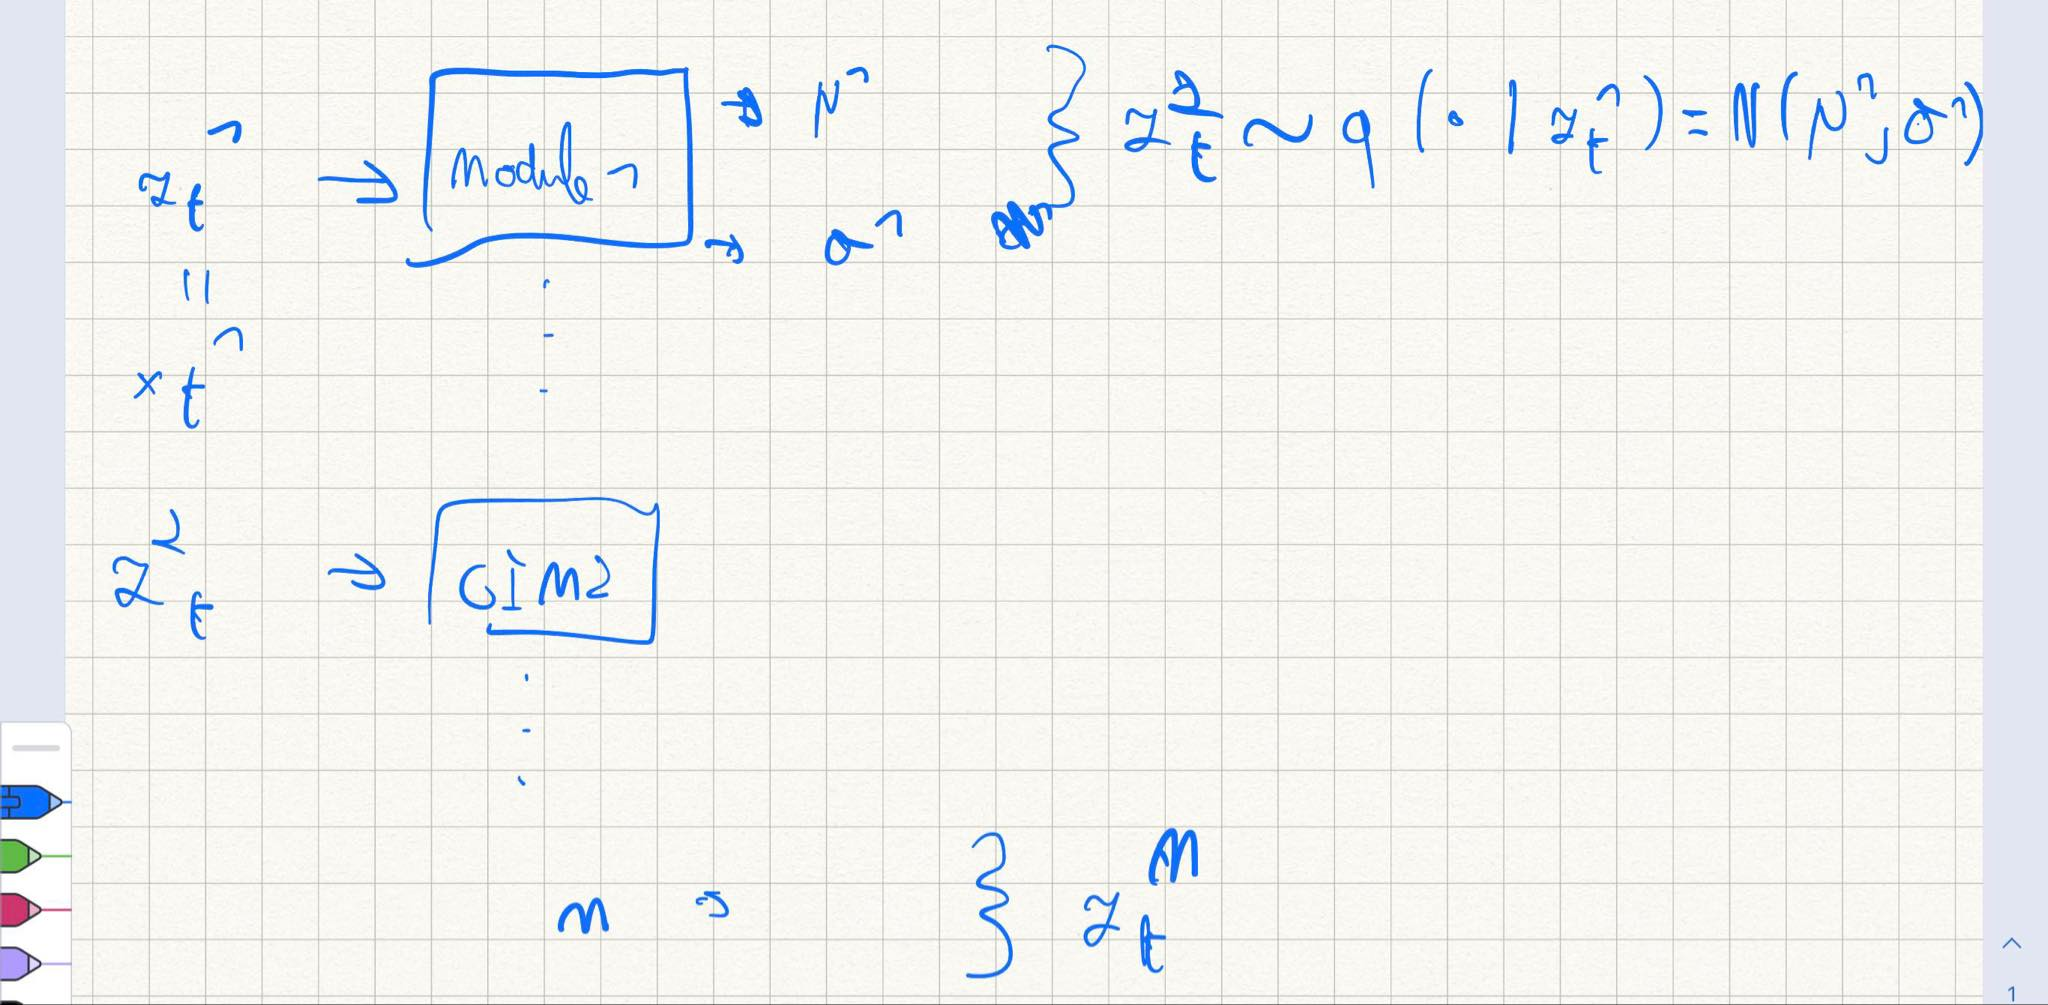
\includegraphics[width=0.7\linewidth]{temp_variational_gim}
				\caption{}
				\label{fig:variationalgim}
			\end{figure}
			
			\begin{align*} % g_enc1, ...
				g_{enc}^1(\xt) &= \zt^1 \\
				g_{enc}^m(\zt^{m-1}) &= \zt^m \\
				g_{ar}(\z_1^M ~ \dots ~ \zt^M) &= \ct
			\end{align*}
			
			The final representation $\ct$ is obtained by propagating $\xt$ through each modules as follows:
			$$ g_{ar}(g_{enc}^M ( \dots	g_{enc}^2(g_{enc}^1(\xt)))) $$
			
			% TODO: WANNEER OVER GRADIENTS BEGINT, A SINGLE MODULE IS DEFINED AS FOLLOWS.. MET F(z m-1) -> (mu, sigm)
			
			
					
		% Distributions
			Additionally, taking inspriation from VAEs, the outputs from $\gencm$ and $\gar$ are in fact samples from a distribution denoted by $q(\zt^m \mid \zt^{m-1})$, defined as a multivariate Gaussian with diagonal covariance matrix, as follows:
			$$\sampleqdot{\zt^{m-1}} = \normalfatmusigma$$
			with $\mufat$ and $\sigmafat$ dependent on $\zt^{m-1}$, specified in more detail in a following subsection.
			The outputs for $\gencm$ and $\gar$ are obtained by sampling from this distribution, denoted respectively, as follows:
 			\begin{align} % z ~ q AND c ~ q
			 	\sample{\zt^m}~ & \qfromzmneg  \label{eq:sample_z_from_q} \\
			 	\sample{\ct}~ & \qfromzM
			 \end{align}
			Modules are thus stochastic and computing $g_{enc}^m(\zt^{m-1})$ twice will likely result in two different representations of $\zt^m$. This is in contrast to CPC and GIM's encodings which remain fixed depending to the input \cite{oordRepresentationLearningContrastive2019, lowePuttingEndEndtoEnd2020}.
		
		% How distributions: predict q + sample
			We achieve these stochastic modules by defining each module $\gencm$ consisting of two blocks. The first block receives as input $\zt^{m-1}$ and predicts the parameters $\mufat$ and $\sigmafat$. These two parameters describe the distribution $\qfromzmneg$. Since we defined $q$ as Gaussian with a diagonal covariance matrix, the distribution can be fully described by those two vectors. The second block samples 
			$\sample{\zt^m} \sampleqdot{\zt^{m-1}}$ from this distribution and produces an output representation. This is depicted in figure \ref{fig:single_variational_module}.
			
			\begin{figure}[h] % img: single module
				\centering
				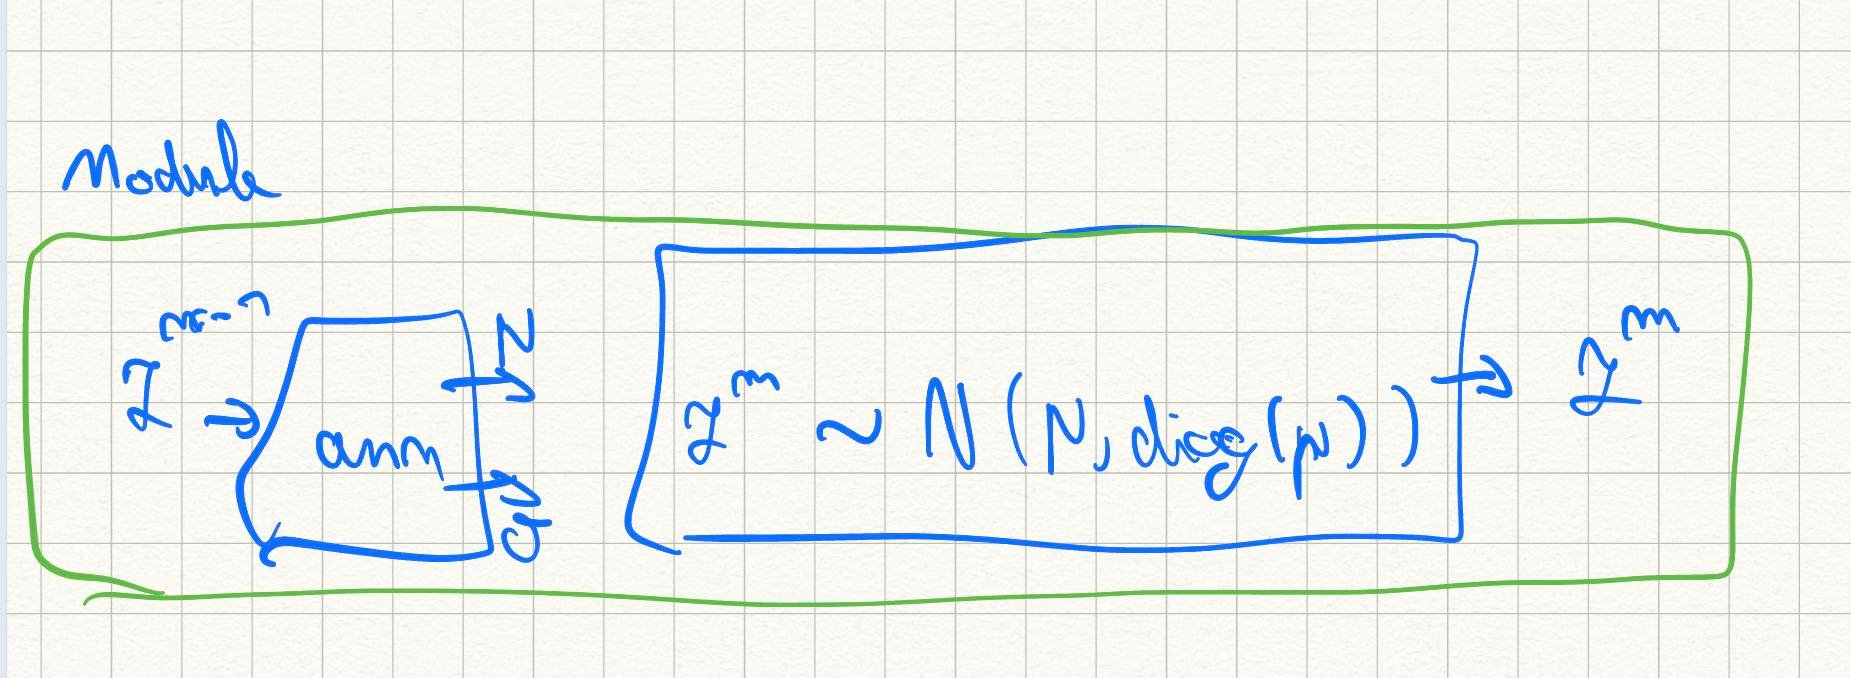
\includegraphics[width=0.7\linewidth]{temp_variational_module}
				\caption{}
				\label{fig:single_variational_module}
			\end{figure}
			
		% define ztm~q() = gaussian., --> z = mu + sigma*noise
			In practice, sampling from $q$ is achieved through a reparametrisation trick, as introduced in \cite{kingmaAutoEncodingVariationalBayes2022}. The equation to compute $\zt^m$ then becomes:
			\begin{equation*}
				\zt = \mufat + \sigmafat \odot \epilonfat
			\end{equation*}
			where $\epilonfat$ corresponds to a sampled value $\samplestandardnormal{\epilonfat}$ and $\odot$ is element-wise multiplication. The procedure to obtain $\ct$ is analogous to $\zt^m$ which we described above.
			
			
		Because of this probabilistic approach, a single patch of data $\xt$ will have multiple representations $\zt^M$, providing increased variance in the representations. This can potentially benefit downstream tasks, particularly when labelled data in scarce \cite{weiRecentAdvancesVariational2021}, leading to improved performance. % TODO: this benefit should be moved to benefits section.
			

		
		
\section{The learning objective}
	Instead of training the neural network end-to-end with a global loss function, the network is split up into modules, which each are optimised greedily with their own personal loss function. Through the introduction of the novel \textit{Variational-InfoNCE} loss, mutual information between temporally nearby representations is maximised, while regularising the latent space to be approximate to the standard Gaussian $\standardnormal$. The Variational-InfoNCE loss is defined as follows:
	
	\begin{equation} % variational_gim_loss % TODO: die k's is niet echt correct/onvolledig
		% \mathcal{L}(\ztk^{m-1}, \zt^{m-1}) = 
		\Lvnce^m =
		\underbrace{\reconstrgim}_{\text{Maximise } I(\ztk^m, \zt^m)} + \underbrace{\beta ~ \latentspaceconstraintgim}_{\text{Regularisation}}
		\label{eq:variational_gim_loss}
	\end{equation}

	$m \in \naturalset$ refers to the $m$'th module. $k \in \naturalset$ corresponds to the number of patches in the future the similarity score $\fkm$ must rate. $\ztk^m$ and $\zt^m$ are encoded samples produced by $g_{enc}^m(\ztk^{m-1})$ and $g_{enc}^m(\zt^{m-1})$, respectively. $X$ is a set of samples ${ \left\{ \ztk^m, \z_1^m, \z_2^m, \dots \right\} }$ where $\zj^m \neq \ztk^m$ are random samples.


	The similarity score $f_k^m(\cdot)$'s definition is identical to \cite{lowePuttingEndEndtoEnd2020}:
	
	$$ f_k^m(\ztk^m,\zt^m) = \exp({\ztk^m}^TW_k^m\zt^m) $$
	
	$\Lvnce^m$ consists of two terms. The first term ensures that encodings of temporally nearby patches contained maximised mutual information. The second ensures that those encodings are all close to the standard normal $\standardnormal$. Finally, $\beta$ is a hyper-parameter which decides the relative importance between the two terms. $\beta >> 1$ will weight more importance to regularisation, but may result in posterior collapse \cite{lucasUnderstandingPosteriorCollapse2022}. On the other hand $\beta \approx 0$ will attach more importance to the mutual information maximisation term while forgetting about the regularisation term. When $\beta = 0$, V-GIM is identical to GIM but with an altered neural network architecture which supports probabilistic encodings.
	
	\subsection{Gradient \textbf{TODO}}
		The gradient of the first term in $\Lvnce^m$ can be approximated through mini-batches, and optimised directly in PyTorch. With regards to the second term, since $\qfromzmneg$ is a Gaussian, a closed form solution exists \cite{kingmaAutoEncodingVariationalBayes2022}, the term can be differentiated without approximated method.
		
		
		%Where the KL divergence for a single sample $x^{(i)}$ is approximated as follows:
		% https://arxiv.org/pdf/1312.6114.pdf, from example
		\begin{equation}
			\frac{1}{2}\sum_{j=1}^J \left( 1 + \log((\sigma_j^{(i)})^2) - (\mu_j^{(i)})^2 - (\sigma_j^{(i)})^2 \right) 
		\end{equation}
		
		\begin{equation} % REAL BUT MUST REMOVE THE (i)	
			\kl{\normal}{\standardnormal} = \latentspaceconstraintclosedform
		\end{equation}
		
		
		where $z^(i,l) = \sigma ^{(i)} \odot \epsilon^{(l)}$ and $\epsilon^(l) \mathcal{N}(0, I)$
		
		\textbf{todo: variables should maybe be bold.}
		
		
		%	TODO: DUS DIE KL DIVERGENCE CLOSED FORM NOTATIE, MAAR BIJ SAMPLING ZOU OOK DEFINITIE VAN Z = MU + SIGMA*ERR GEVEN
	
	
	\subsection{Continuous space around the origin} \label{cha:contin_space}
		% around N()
			As we discussed earlier, the representations or encodings $\sample{\zt^m}~ \qfromzmneg$ generated by each module $m$ are samples from a Gaussian distribution (which may not necessarily be the standard normal). These samples are optimised to be as close as possible to the standard normal $\standardnormal$. 
	
		% smooth changes
			Consider $\ztk^{m-1}$ and $\zt^{m-1}$ which each serve as input for a fully trained module $\gencm$. These two inputs are temporally nearby, and thus, due to the slowly varying features assumption \cite{zhangSlowFeatureAnalysis2012} have a lot of information in common. This means that the correspondence score of their encodings, estimated by the scoring function $\fkmblank$, should also be high. However, as depicted in \ref{fig:gaussian-neighbourhood}, the encodings for $\ztk^{m-1}$ correspond an entire space $ \{ {\ztk^m}^{'},~{\ztk^m}^{''},~\dots \}$ centred around a particular mean vector $\mufat$. If $\Lvnce^m$ is optimal, this means that given encoding $\zt^m$, $f_k^m({\ztk^m}^{'}, {\zt^m})$ should be  large, but also $f_k^m({\ztk^m}^{''}, {\zt^m})$, while remaining small for random encodings $\zi^m \neq \ztk^m$. The correspondence scores must thus be similar for all encodings in a particular neighbourhood, meaning they all have similar mutual information to $\zt^{m}$. This is important, because it will ensure smooth transitions in the latent space. Furthermore, optimising this loss function also maximises the mutual information between outputs of successive modules $I(\zt^{m-1}, \zt^{m})$ \cite{lowePuttingEndEndtoEnd2020}, and the smooth transitions will reflect on the original representations $\xt$.			 
		
		\begin{figure} % gauss neighbourhood
			\centering
			\includegraphics[width=0.7\linewidth]{"gaussian neighbourhood"}
			\caption{}
			\label{fig:gaussian-neighbourhood}
		\end{figure}
		
		% gaps
			Finally, since the set of encodings $ \{ {\zt^1}^{'},~{\zt^1}^{''},~\dots \}$ from a single patch $\xt$ corresponds to a large neighbourhood in the latent space, and since the latent space is fairly small (standard normal) representation distributions from different data points are likely to be pushed around, trying to utilise the limited space as best as they can. This results in a less likely chance of obtaining holes in the latent space.
			
			The end result is a continuous space around the origin, which is a crucial observation. It will serve as the main argument for why V-GIM's representations are interpretable, while traditional techniques such as CPC and GIM do not have these guarantees. 

			


		
	
	
	
\section{Computational benefits}
	Each module in V-GIM is greedily trained through the variational InfoNCE loss. As a result many of GIM's computational benefits of greedy self-supervised learning introduced, such as memory-efficient asynchronous distributed training and reduction of the vanishing gradient problem \cite{lowePuttingEndEndtoEnd2020}. However, additionally, latent space constraints are posed on the outputs from each module, which will show benefits which are not only applicable to the final module's outputs but also in between modules.
	

	
\subsection{Representations}
	\subsubsection{Interpretability of final and intermediate representations}
	
		By carefully optimising the latent space with the properties discussed in section \ref{cha:contin_space}, results in a space where sampling from a point around the origin is likely to correspond to a data point which is similar to the dataset. If a decoder is trained on this space and a latent representation is chosen that the decoder has never seen before, it will generalise well to unseen data. This is in contrast to GIM and CPC which do not pose constraints on the latent space. Although a decoder can also be trained on GIM or CPC's encodings, which generalises well to a validation set, the latent space is highly unpredictable and sampling a random encoding around the origin is not guaranteed to result in a meaningful decoding as it may be a representation which is very dissimilar to the ones the decoder was trained on, hence not generalising well to these representations. We depict this in figure \ref{fig:no-regularisation}. Without a regularisation, the shape of the latent space is unpredictable, and thus we do not known what from which data points samples are taken when choosing a random latent representation, or when interpolating between two well formed latent representations (aka, two encodings from the dataset).
	
		\begin{figure} % regul vs no regul
			\centering
			\includegraphics[width=0.7\linewidth]{"no regularisation"}
			\caption{Left is without regularisation (eg space obtained from a single module from GIM). Right is with regularisation (eg: V-GIM). A decoder's objective is to learn a reversed mapping function from the blue z-space to the green x-space. The decoder is only trained on the blue cloud and not data points around it so it may not generalise well to those representations. }
			\label{fig:no-regularisation}
		\end{figure}
	
		
		This is a very important observation and has great implications on V-GIM's interpretability, compared to traditional techniques such as CPC and GIM. Not only can we assess the information contained in an encoding through a decoder, we can even attempt to understand the underlying structure of the encodings.
		
		Similar to VAE's, given a sample in the latent space around the origin, we can move this point in a particular direction in a particular dimension and observe the effect through the decoder.
		
		Finally, since V-GIM's neural network architecture consists of a variable number of modules, which each generate interpretable encodings, the repre
		
		possible observing different levels of abstractions contained in encodings at different levels.
			
		This is in contrast to VAE which only results in transparent final representations.		
			- ALSO NO EXPLICIT NEED FOR A DECODER. THIS REMAINS, SO ARCH CAN BE SIMPLER.
	
	
	\subsubsection{Improved generalisation through representation variance}
	
	Better generalisation for downstream tasks
		- Overfitting: reduction of required labelled data needed. Similar data is similar region, the kl divergence makes regions bigger.
		% copied from a bit higher
		% Because of this probabilistic approach, a single patch of data $\xt$ will have multiple representations $\zt^M$, providing increased variance in the representations. This can potentially benefit downstream tasks, particularly when labelled data in scarce \cite{weiRecentAdvancesVariational2021}, leading to improved performance. % TODO: this benefit should be moved to benefits section.

		Overfitting during inference:
		- The same datapoint has multiple (similar) representations, such that learning techniques for downstream tasks will not be able to "memorise" the latent space as easily.
		
		- Holes: more predictable inference, such that unseen data is more likely to be near clusters. And thus downstream tasks receive latents that are more similar to what is seen before.
		= better generalisation
		

	\subsubsection{Batch normalisation mechanism}
	Batch normalisation: is useful for following modules, BUT ALSO DOWNSTREAM TASKS!
		- built in batch normalisation mechanism
		- During training similar behaviour to batch normalization in-between layers
	
	- Independent latent dimensions
		

	
	
	
	

	







%\textbf{Other sources:} \\
%!!! Abstract on VAE: The fundamental idea in VAEs is to learn the
%distribution of data in such a way that new meaningful data with more intra-class variations can be generated
%from the encoded distribution.
%The ability of VAEs to synthesize new data with more representation variance
%at state-of-art levels provides hope that the chronic scarcity of labeled data in the biomedical field can be
%resolved.
%--> and thus for downstream tasks, has a way of obtaining more labelled data? --> better generalisation


%The goal of representation learning is to be useful for downstream tasks. The most important meta-prior is called ‘disentanglement’ which is an unsupervised learning technique that breaks down, or disentangles, each feature into narrowly defined variables and encodes them as separate dimensions 

%Intuitively, a factorial code disentangles the individual elements that were originally mixed in the sample, just as
%humans recognize complex things by disentangling independent elements. If the dimensions of the latent vector are
%independent of each other, it is factorial disentangled, i.e., a
%good representation. VAEs have made such nonlinear latent
%variable models tractable for modeling complex distributions,
%and efficient extraction of relevant biological information
%from learned features for biological data sets, referred to as
%unsupervised representation learning
%https://ieeexplore.ieee.org/stamp/stamp.jsp?tp=&arnumber=9311619








%We show that the Beta-VAE outperforms principal component analysis (PCA) and learns interpretable and independent representations of the generative factors of variance in the spectra %https://pubs.acs.org/doi/pdf/10.1021/acs.jpclett.2c01328
%



\chapter{Experiments}

In this chapter we assess the encodings obtained from Variational Greedy Infomax (V-GIM) and compare results against its non-variational counterpart (GIM). We train the encoders on sequential data from the audio domain and assess the quality of the representations. The assessment is achieved by transforming the latent space into a two-dimensional space using t-SNE and observing clusters. Additionally, the representations obtained from the encoders are used as input for a linear classifier, whose accuracy scores provide insights in the representations' performance.

Additionally, we gather more insights in the representations. We assess the amount of labelled data required for obtaining adequate performance in downstream tasks, by training the linear classifier on smaller subsets of the dataset. Finally, we provide insights in the interpretation of the latent features, by developing a decoder for V-GIM's encodings. We can then observe the information that is contained in each of the representation's components by altering values and observing the produced output of the decoder. 


%- Experimental details encoder:
%	- Learning task: to find representations for speech data.
%	- Dataset:
%		- full data + split up
%	- Architecture
%- Results
%	- Loss functies
%	- Linear separability (t-sne)
%	
%- Generalisation (generalisation)
%		- Accuracies Subsets
%- Interpretability
%		- Encoder distributions (shows that interpolation can make sense)
%		- Decoder: loss, architecture

	






% TODO: I CALL IT Variational Greedy Infomax: V-GIM

\section{Experimental details encoder}

	
	
	\subsection{Dataset}
		The Greedy Infomax model is trained on speech data. The model takes as input a raw speech signal of a fixed length and outputs a latent representation for that signal. The dataset is split up into 729 training files and 122 test files. In each file consists of a single spoken sound consisting of three consonants and three vowels, where the consonants and vowels alternate each other. Some Examples are the sounds "gi-ga-bu" and "ba-bi-gu". All the sounds are spoken by the same person, at a constant and peaceful \textbf{todo: describe emotional aspects of speech audio}. 
		
		The following transformations are applied to the audio files. Although the original contains a sample rate of 441 Khz, the audio files are downsampled to 16 Khz, matching the sample rate used by Löwe \cite{lowePuttingEndEndtoEnd2020}. This significantly reduces the size of the latent representations, and thus the required amount of VRAM during training. Additionally, two types of noise are added to the data. We apply Gaussian white noise, at different decibels ranging between zero and fifteen \textbf{TODO ...}.
		
		- also background noise from dataset. is a way to enlarge our dataset. 
		- Each audio file is cut to have length \textbf{10240}. Additionally, 
		
		
		Splitting: see appendix  \ref{appendix:split_syllables}
		
	\subsection{Architecture}
		% cnn + gru: so inputs can have variable lengths
			Training is done speech signals of fixed length, eg 8,800 samples. Notice however, that the neural network only makes use of convolutional neural networks layers and GRU's, no fully connected layers. The input dimensions can therefore be variable during inference. Only the number of channels in the latent representations should be constant, but the length can change.
			
		\begin{figure}[h]
			\centering
			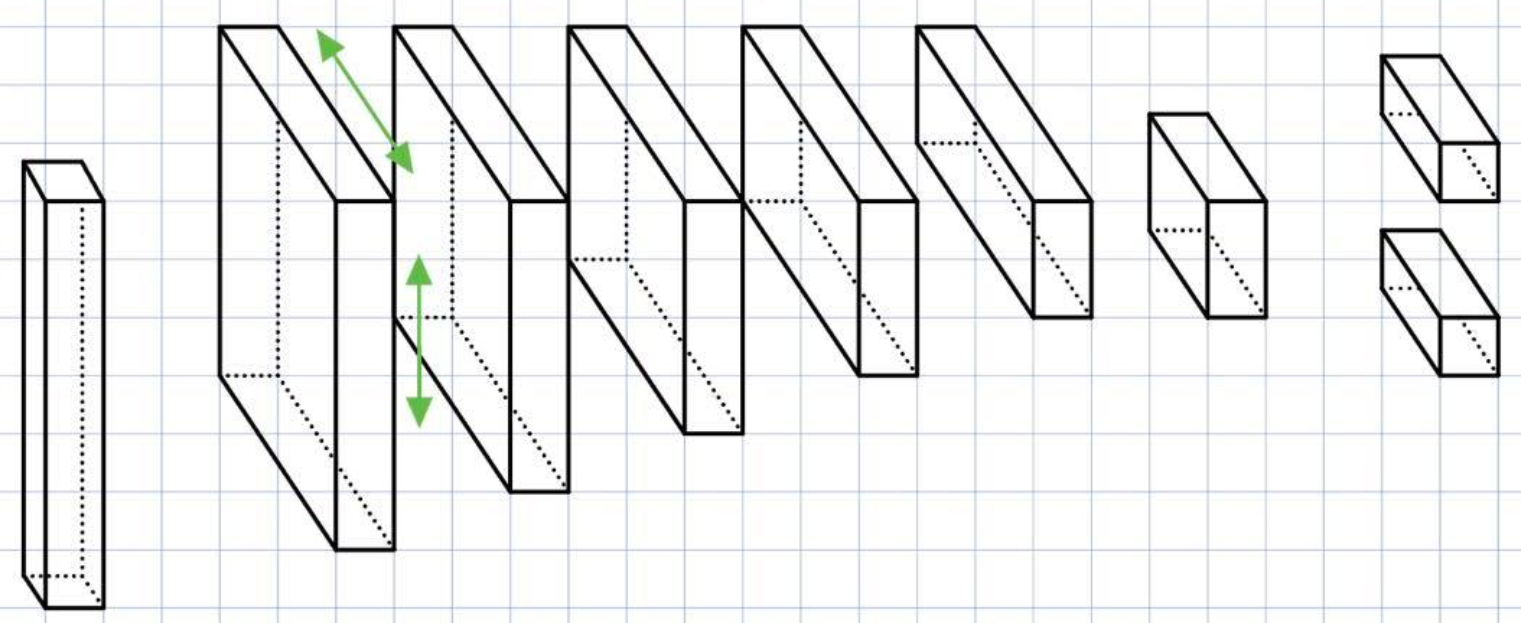
\includegraphics[width=0.7\linewidth]{architecture}
			\caption{}
			\label{fig:architecture}
		\end{figure}
	
		Figure \ref{fig:architecture} displays how via contrastive predictive coding an input speech signal is transformed into two latent vectors. The two vectors combined describe a Gaussian distribution for each feature of the latent representation. One vector corresponds to the means and the other to the standard deviations of the latent distributions. We variational autoencoders assume independent latent features, such that the covariance matrix is non negative on the diagonal and zero off the diagonal. This allows the covariance matrix to be discribed using a single vector. We again, make use of this (plausible incorrect?) assumption of having independent latent features.




		% Training on longer patches, classification on padded sub-patches.
		During inference, (in this context obtaining the latent representations for our input signals), depending on the length of the input signal, the length of the output latent representation will differ.
		If we wish to look at how separable latent representations are for syllables, the length can be variable. Some input sounds could be 6,600 samples, while others 8,800 samples. We therefore pad the syllables with zeroes in front and end of the signal, to obtain fixed length of equal to that of the longest syllable; 8,800 samples.
		
		Training happens on longer data samples, and every \textbf{X} epochs t-SNE visualisations are made to observe evolutional of dis-entanglement.
		

\section{Results}

	% Enkele loss curces etc
	\subsection{Results CPC Simple v2 w/ 2 modules}
	
	\subsection{Distributions}
	
	% loss func only shows part of picture -> towards tsne
		Although loss is used as evaluation metric, it only shows part of the picture. The main objective for the representations is to obtain some form of "decoupled/dis-entanged" features that are more easily separable. This evaluation is done by projecting the latent representations to a 2D plane, via t-SNE. Then datapoints are coloured in depending on their the syllable that was pronounced, eg: "gi" or "ga".
		
		
		

		%Graphs t-sne: Beta = 0	
		%	\begin{figure}[h]
		%		\centering
		%		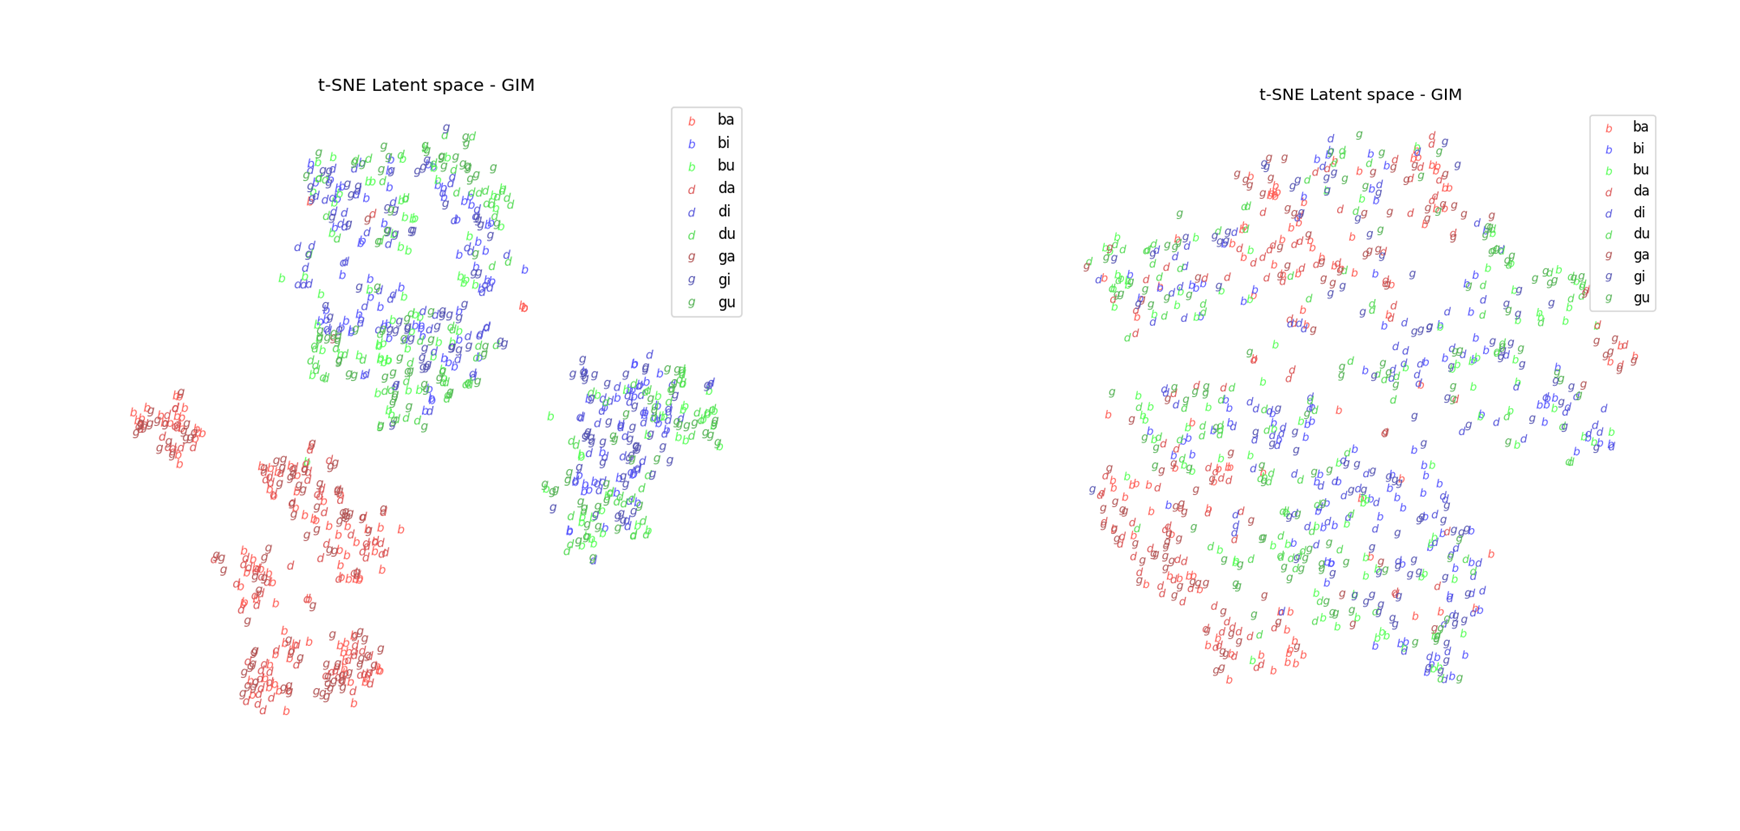
\includegraphics[width=0.7\linewidth]{screenshot023}
		%		\caption{}
		%		\label{fig:tsne_two_module_kld_0}
		%	\end{figure}
		%	
		%	
		%	\begin{figure}[h]
		%		\centering
		%		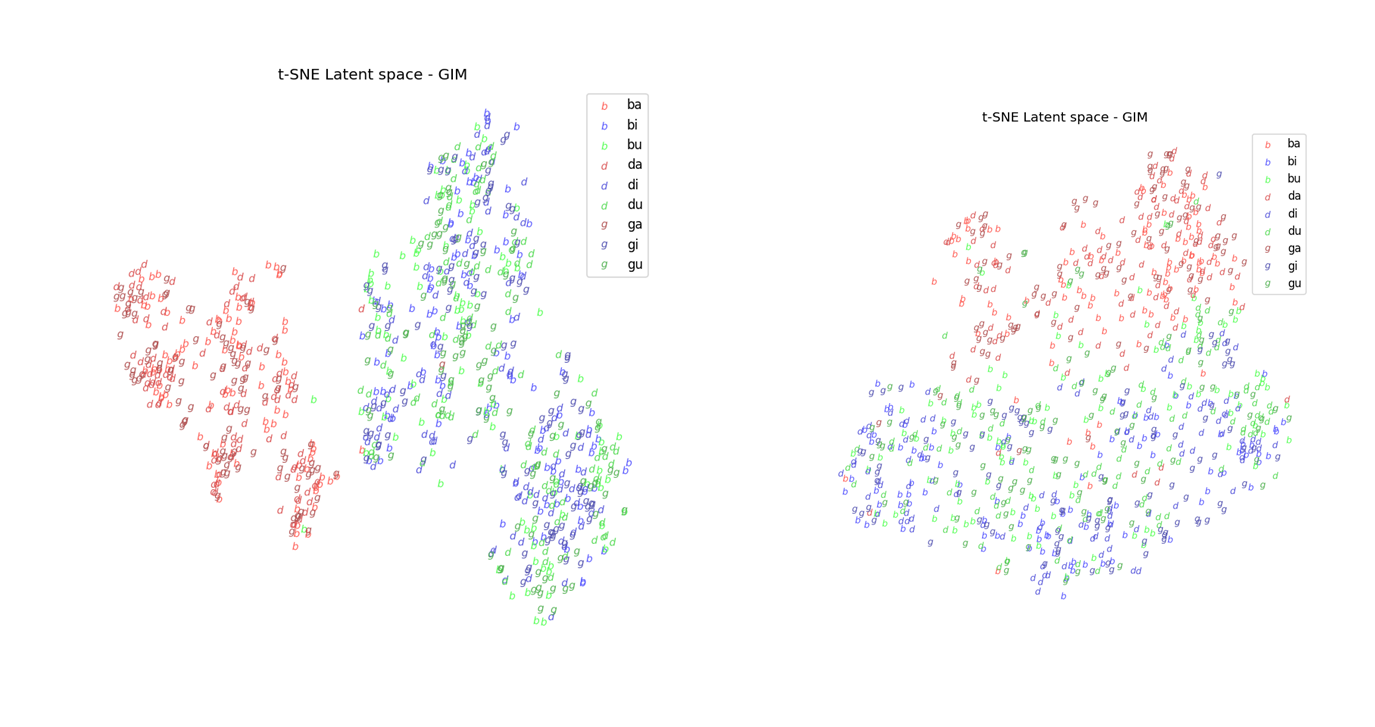
\includegraphics[width=0.7\linewidth]{screenshot024}
		%		\caption{}
		%		\label{fig:tsne_two_module_kld_0033}
		%	\end{figure}
	
	%	
	%	\ref{fig:tsne_two_module_kld_0}: can see that second model harms performance. We believe this can be explained via the learning rate. \ref{fig:tsne_two_module_kld_0033}, there we see that second module performs better separation, indicating that the intermediate KL convergence constraint (causing the normal Gaussian distributions) also serves as a batch normalisation term, and thus resulting in faster convergence.
	%
	%	
	%	---------------------------------------------
	%	
	%	\textbf{T-sne visualisations:}
	%	Multiple models trained, trained GIM, but single module (exact CPC architecture), one with autoregressor and once without autoregressor layer, so only CNN layers. 200 epochs, trained on split up data samples.
	%	
	%	1) Only CNN: We observe better linear separability
	%	\begin{figure}[h]
	%		\centering
	%		\includegraphics[width=0.7\linewidth]{"cpc architecture ONLY CNN t-SNE_latent_space_GIM"}
	%		\caption{}
	%		\label{fig:cpc-architecture-only-cnn-t-snelatentspacegim}
	%	\end{figure}
	%	
	%	2) CNN + 1 autoregressor layer:
	%	\begin{figure}[h]
	%		\centering
	%		\includegraphics[width=0.7\linewidth]{"cpc architecture CNN + GRU t-SNE_latent_space_GIM"}
	%		\caption{}
	%		\label{fig:cpc-architecture-cnn--gru-t-snelatentspacegim}
	%	\end{figure}
	%	
	%	3) This is the pure data visualised (no latent representation).
	%	Were at least doing a bit better than the original data, so that's good! our work is not for nothing.
	%	\begin{figure}[h]
	%		\centering
	%		\includegraphics[width=0.7\linewidth]{"_ t-SNE_latent_space_Original data"}
	%		\caption{}
	%		\label{fig:-t-snelatentspaceoriginal-data}
	%	\end{figure}
	%	
	%	
	%	4) old GIM with all modules each one layer. l1 .. 5 - cnn, l6 = gru. img shows l5 = cnn:
	%	model can more easily distinguish A's from other \textbf{klinkers}. Partly, it kinda makes sense for GIM to learn to separate \textbf{klinkers}. Since they last longer (longer duration), the loss function will more likely randomly sample a subwindow from the "aa's" than from the \textbf{medeklinker} part.
	%	
	
	
	
	
	
	
	
	
	
	
	

%		\begin{figure}
%			\centering
%			\includegraphics[width=0.7\linewidth]{"t-sne kld=0 module 2"}
%			\caption{}
%			\label{fig:t-sne-kld0-module-2}
%		\end{figure}
%		\begin{figure}
%			\centering
%			\includegraphics[width=0.7\linewidth]{"t-sne kld=0.0033 module 1"}
%			\caption{}
%			\label{fig:t-sne-kld0}
%		\end{figure}
%		\begin{figure}
%			\centering
%			\includegraphics[width=0.7\linewidth]{"t-sne kld=0.0033 module 2"}
%			\caption{}
%			\label{fig:t-sne-kld0}
%		\end{figure}
%		\begin{figure}
%			\centering
%			\includegraphics[width=0.7\linewidth]{"t-sne kld=0 module 1"}
%			\caption{}
%			\label{fig:t-sne-kld0-module-1}
%		\end{figure}
	
	
	\subsubsection{T-sne}
	T-distributed stochastic neighbour embedding.
	
	
	Visualising data using T-sne.
	given N high-dimensional objects x1 .. xN. wants to see underlying structure of the data. eg clusters? local structures?
	
	How visiualise very high dimensional data?
	
	Introduction:
		build map where similar data points are moved close to each other and unsimilar points far away. and map in eg 2 or 3 dims. (scatter plot).
		

		
		
		
		
		
		
	

			
			\begin{figure}[ht] % four t-sne images
				\centering
				\begin{subfigure}{0.45\linewidth}
					\centering
					\includegraphics[width=\linewidth]{"t-sne kld=0.0033 module 1"}
					\caption{}
					\label{fig:t-sne-kld33-module1}
				\end{subfigure}
				\hspace{0cm}
				\begin{subfigure}{0.45\linewidth}
					\centering
					\includegraphics[width=\linewidth]{"t-sne kld=0.0033 module 2"}
					\caption{}
					\label{fig:t-sne-kld33-module2}
				\end{subfigure}
				\vspace{0cm}
				\begin{subfigure}{0.45\linewidth}
					\centering					
					\includegraphics[width=\linewidth]{"t-sne kld=0 module 1"}
					\caption{}
					\label{fig:t-sne-kld0-module-1}
				\end{subfigure}
				\hspace{0cm}
				\begin{subfigure}{0.45\linewidth}
					\centering
					\includegraphics[width=\linewidth]{"t-sne kld=0 module 2"}
					\caption{}
					\label{fig:t-sne-kld0-module-2}
				\end{subfigure}
				\caption{My images}
				\label{fig:myimages}
			\end{figure}
		
		
		
		
		
		
		
		
	
	
	
	


	



\section{Generalisation}

	\begin{figure} % two graphs of subsets
		\centering
		\begin{subfigure}[b]{0.4\textwidth}
			\centering
			% graph subsets (module 1)
			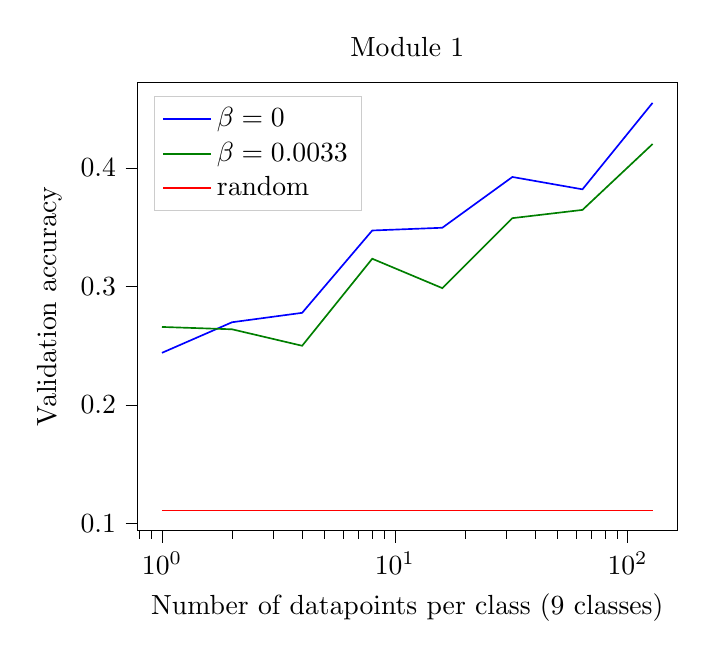
\begin{tikzpicture}
				
				\definecolor{darkgray176}{RGB}{176,176,176}
				\definecolor{green01270}{RGB}{0,127,0}
				\definecolor{lightgray204}{RGB}{204,204,204}
				
				\begin{axis}[
					legend cell align={left},
					legend style={
						fill opacity=0.8,
						draw opacity=1,
						text opacity=1,
						at={(0.03,0.97)},
						anchor=north west,
						draw=lightgray204
					},
					log basis x={10},
					tick align=outside,
					tick pos=left,
					title={Module 1},
					x grid style={darkgray176},
					xlabel={Number of datapoints per class (9 classes)},
					xmin=0.784584097896751, xmax=163.143760296865,
					xmode=log,
					xtick style={color=black},
					y grid style={darkgray176},
					ylabel={Validation accuracy},
					ymin=0.0939236113230387, ymax=0.472048606660631,
					ytick style={color=black}
					]
					\addplot [semithick, blue]
					table {%
						1 0.244047609737941
						2 0.26984125818525
						4 0.277777765819005
						8 0.347222211020333
						16 0.3495370165507
						32 0.392361106872559
						64 0.381944427490234
						128 0.454861106872559
					};
					\addlegendentry{$\beta=0$}
					\addplot [semithick, green01270]
					table {%
						1 0.265873005049569
						2 0.263888875416347
						4 0.249999988419669
						8 0.323412685394287
						16 0.29861110051473
						32 0.357638893127441
						64 0.364583320617676
						128 0.420138854980469
					};
					\addlegendentry{$\beta=0.0033$}
					\addplot [semithick, red]
					table {%
						1 0.111111111111111
						2 0.111111111111111
						4 0.111111111111111
						8 0.111111111111111
						16 0.111111111111111
						32 0.111111111111111
						64 0.111111111111111
						128 0.111111111111111
					};
					\addlegendentry{random}
				\end{axis}
				
			\end{tikzpicture}
			
			%\caption{Caption for the first graph.}
		\end{subfigure}
		\hfill
		\begin{subfigure}[b]{0.4\textwidth}
			\centering
				% graph subsets (module 2)
			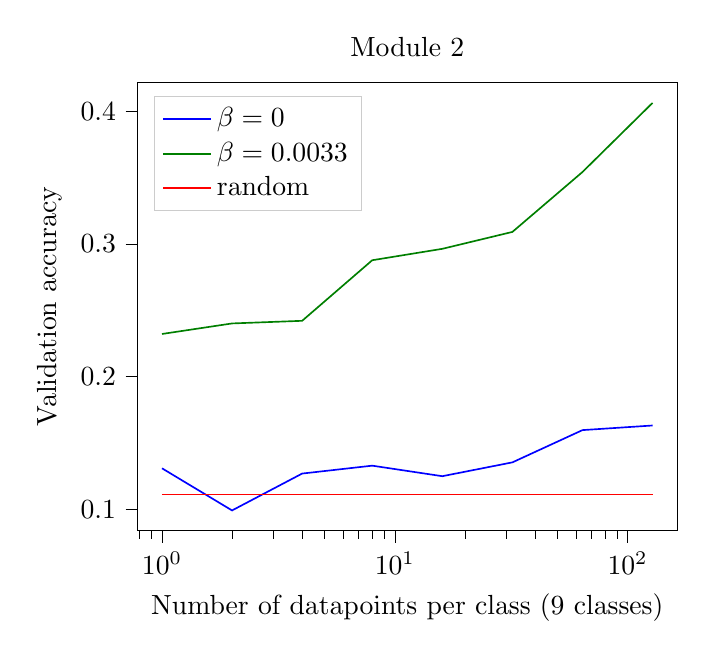
\begin{tikzpicture}
				
				\definecolor{darkgray176}{RGB}{176,176,176}
				\definecolor{green01270}{RGB}{0,127,0}
				\definecolor{lightgray204}{RGB}{204,204,204}
				
				\begin{axis}[
					legend cell align={left},
					legend style={
						fill opacity=0.8,
						draw opacity=1,
						text opacity=1,
						at={(0.03,0.97)},
						anchor=north west,
						draw=lightgray204
					},
					log basis x={10},
					tick align=outside,
					tick pos=left,
					title={Module 2},
					x grid style={darkgray176},
					xlabel={Number of datapoints per class (9 classes)},
					xmin=0.784584097896751, xmax=163.143760296865,
					xmode=log,
					xtick style={color=black},
					y grid style={darkgray176},
					ylabel={Validation accuracy},
					ymin=0.0838541626930237, ymax=0.421602182728904,
					ytick style={color=black}
					]
					\addplot [semithick, blue]
					table {%
						1 0.130952375956944
						2 0.0992063454219273
						4 0.126984120096479
						8 0.132936503546579
						16 0.124999993642171
						32 0.135416660308838
						64 0.159722213745117
						128 0.163194446563721
					};
					\addlegendentry{$\beta=0$}
					\addplot [semithick, green01270]
					table {%
						1 0.23214284828731
						2 0.240079355239868
						4 0.242063480785915
						8 0.287698405129569
						16 0.296296278635661
						32 0.309027767181396
						64 0.354166641235352
						128 0.40625
					};
					\addlegendentry{$\beta=0.0033$}
					\addplot [semithick, red]
					table {%
						1 0.111111111111111
						2 0.111111111111111
						4 0.111111111111111
						8 0.111111111111111
						16 0.111111111111111
						32 0.111111111111111
						64 0.111111111111111
						128 0.111111111111111
					};
					\addlegendentry{random}
				\end{axis}
				
			\end{tikzpicture}
			
			
			%\caption{Caption for the second graph.}
		\end{subfigure}
		\caption{Validation accuracy for different subset sizes}
	\end{figure}


	


\section{Interpretability}

	\subsection{Decoders for Variational Greedy InfoMax}
		% investigate what info in V-GIM + argue can interpolate
		To investigate what information is contained in V-GIM's representations, we train a decoder on top of each of V-GIM's modules. Contrary to variational autoencoders, V-GIM is fully independent from the decoder and does not require one for training. Furthermore, we analyse the underlying structure the representations obtained from each module. This is achieved by altering representation's component values and observing the effects through the decoder. As we argued in the previous section, this is only possible because V-GIM's encodings is optimised to be approximate to the standard normal. As long as this is case, there are no "gaps" in the latent space around the origin. The decoder will be able to generalise to the altered representations as long as the representations are close to the origin.
		
		We train a decoder for each of V-GIM's modules. As such we can assess the information contained in the final representation, but also the representations of intermediate modules.
		
		% result:
		timesteps in second module captures much wider time frame and first module, so observes different content.
		first module: each component respoble for different frequency.
		
		second module:
		combination of frequencies.
		
		\subsubsection{Decoder architecture}
		We develop two decoders, one for each module. 
		$$
			\text{decoder}^1(\zt^1) = \xt
		$$
		$$
			\text{decoder}^2(\zt^2) = \xt
		$$
		Both decoders' architectures are symmetric to the architecture the V-GIM's encoder. Where the convolutional and max pooling layers are both replaced by transposed convolution layers.
		The architecture for 
		
		\begin{tabular}{|c|c|c|c|}
			\hline
			Layer & Filter size & Stride & Padding \\
			\hline
			TransConv1 & 3 & 1 & 1 \\
			\hline
		\end{tabular}
	
	
	
		% -----
		The decoder consists of a convolutional neural network which takes as input the encodings from V-GIM and is tasked to reconstruct the original data. The decoder is optimised to minimise the mean squared error between mel spectrograms of the original data and the reconstructed data. 
		
		We optimise the decoder with the loss function introduced in [cite] and alter it to use mel spectrograms to better capture the important speech features according to the auditory system. The loss function we use is the following:
		$$
		\mathcal{L}_{\text{decoder}} =\frac{1}{n} \sum_{i=1}^n\left( \log (MEL(y^{(i)})) -\log (MEL(\hat{y} ^{(i)} )) \right)^2
		$$
		
		
	
	
	
	
	% first module:
	
%	class SimpleV2Decoder(GimDecoder):
%	def __init__(self, hidd_channels=32, out_channels=1):
%	super().__init__("Simple_v2_DECODER")
%	
%	# Encoder architecture (Simple v2)
%	kernel_sizes = [10, 8, 3]
%	strides = [4, 3, 1]
%	padding = [2, 2, 1]
%	max_unpool_k_size = 8
%	max_unpool_stride = 4
%	
%	# Decoder architecture
%	self.decoder = nn.Sequential(
%	nn.ConvTranspose1d(hidd_channels, hidd_channels,
%	kernel_sizes[2], stride=strides[2], padding=padding[2]),
%	nn.ReLU(),
%	
%	# Replaces maxpooling
%	nn.ConvTranspose1d(hidd_channels, hidd_channels, max_unpool_k_size,
%	stride=max_unpool_stride, padding=0, output_padding=0),
%	nn.ReLU(),
%	
%	nn.ConvTranspose1d(hidd_channels, hidd_channels,
%	kernel_sizes[1], stride=strides[1], padding=padding[1], output_padding=1),
%	nn.ReLU(),
%	
%	# Replaces maxpooling
%	nn.ConvTranspose1d(hidd_channels, hidd_channels, max_unpool_k_size,
%	stride=max_unpool_stride, padding=0, output_padding=3),
%	nn.ReLU(),
%	
%	nn.ConvTranspose1d(hidd_channels, out_channels,
%	kernel_sizes[0], stride=strides[0], padding=padding[0], output_padding=2),
%	)
%	
%	def forward(self, x):
%	return self.decoder(x)
	
	
	


% Second module:
%
%class SimpleV3DecoderTwoModules(GimDecoder):
%def __init__(self, hidd_channels=32, out_channels=1):
%super().__init__("Simple_v3_2Module_DECODER")
%
%kernel_sizes = [6, 6, 3]
%strides = [2, 2, 1]
%padding = [2, 2, 1]
%
%self.module2 = nn.Sequential(
%nn.ConvTranspose1d(hidd_channels, hidd_channels,
%kernel_sizes[2], stride=strides[2], padding=padding[2]),
%nn.ReLU(),
%nn.ConvTranspose1d(hidd_channels, hidd_channels,
%kernel_sizes[1], stride=strides[1], padding=padding[1], output_padding=0),
%nn.ReLU(),
%nn.ConvTranspose1d(hidd_channels, hidd_channels,
%kernel_sizes[0], stride=strides[0], padding=padding[0], output_padding=0),
%)
%self.module1 = SimpleV2Decoder(hidd_channels, out_channels)
%
%def forward(self, z):
%z = self.module2(z)
%x = self.module1(z)  # SimpleV2Decoder
%return x

	
	
		\subsubsection{Loss function}
		
 % We use five convolutional layers with strides [5, 4, 2, 2, 2], filter-sizes [10, 8, 4, 4, 4] and 512 hidden units with ReLU activations.
	



	
	
	\subsection{Decoder: predictions on test set}
	Fig \ref{fig:bagidi1-model29-true-vs-predicted} displays the reconstructed signal from the vocal sound "ba-gi-di". The two images on the left displays the original signal, while the right two images contain the reconstructed signal.  The upper images displays the signals in time domain, the bottom images spectral domain. The reconstructed signal is an audio sample, for instance which is encoded via Greedy Infomax (up to the fourth (and final) convolution layer), this output is then given to a decoder to reconstruct the original signal.
	
	%TODO: BROKEN 
	%\begin{figure}[h]
	%	\centering
	%	\includegraphics[width=0.7\linewidth]{"../../../../../../../../../GitHub/thesis-fabian-denoodt/GIM/logs/GIM_DECODER_experiment/MSE + scFFT Loss FFT=10240 Lambda=1.0000000/lr_0.0010000/GIM_L4/predictions_model=29/test/bagidi_1, model=29, True vs Predicted"}
	%	\caption{Top left: original, time domain. Bottom left: original }
	%	\label{fig:bagidi1-model29-true-vs-predicted}
	%\end{figure}




%(van die YT VID) + book: https://christophm.github.io/interpretable-ml-book/neural-networks.html
%What about internals (look at neural representations):
%Our method is more like this approach, both explaining internals
%- feature visualisation
%focus on specific neuron, and use it to generate images to activate it.
%use the behaviour of that model and find image that activates the neuron.
%-> isolate neurons that detect textures etc.
%(distill.pub/2017/feature-visualisation, distill/2021/multimodal-neurons)
%
%
%
%%Additionally, researchers have explored methods to explain black box models.
%%- Relevance weighting, ... 

%^^ hun prentjes die ze genereren die de maximum activatie generenen, zijn geen echte prentjes, en zou wrs niet even goed interpreteerbaar zijn voor audio data, vermits her oor gevoeliger is voor disturbance en dus minder goed kan verstaan.
%*******************************************************************************
\chapter{Relation to existing work} \label{cha:5}

We have studied the representations obtained by maximising the InfoNCE loss function. We achieved this through the addition of a regularisation term to the loss function, resulting in a space that is easier to analyse and understand. In this chapter, we give an overview of the existing literature that is relevant to our research. We begin with a discussion of representation learning techniques related to mutual information maximisation, and slowly digress into interpretable representations. Furthermore, we give an overview of the existing regularisation techniques used for both improved generalisation and better representations. Finally, we give an overview of alternative priors that have been introduced to the VAE framework in the past decade.


\section{Mutual information and interpretable representation learning}
	%\cite{lowePuttingEndEndtoEnd2020}
	%\citep{lowePuttingEndEndtoEnd2020}
	%\citeyear{lowePuttingEndEndtoEnd2020}

	V-GIM is based on the ideas of mutual information maximisation introduced in CPC and GIM \citep{lowePuttingEndEndtoEnd2020, oordRepresentationLearningContrastive2019}. This is achieved by maximising the mutual information between temporally nearby patches, assuming common information between nearby data \citep{lowePuttingEndEndtoEnd2020}. Similar approaches utilising mutual information maximization for representation learning have also been explored.
	
	Deep InfoMax incorporates an ANN encoder which maximises the mutual information between input and output. This is achieved by incorporating knowledge about locality in the representations, resulting in locally-consistent information across structural locations \citep{hjelmLearningDeepRepresentations2019}. Meanwhile, InfoGAN, C-DSVAE and S3VAE each introduce a different flavour on the mutual information maximisation scheme, while obtaining disentangled representations \citep{chenInfoGANInterpretableRepresentation2016, baiContrastivelyDisentangledSequential2021, zhuS3VAESelfSupervisedSequential2020}. 
	
	In addition, InfoGAN's learning approach results in interpretable representations. Manipulating an individual dimension in the latent space results in changes to a specific feature of the generated data while leaving other features unaffected. This approach is similar to how V-GIM achieves interpretability using an optional decoder. However, V-GIM takes this a step further by composing its architecture into one or more modules, each with their own interpretable representations. This enables the understanding of the final representations, but also the internal parts of the neural network, providing increased interpretability.
	
	Building upon InfoGAN's concepts, Bridge-GAN introduces an intermediate latent space, or ``bridge" between text and images. This approach enables the synthesis of interpretable and disentangled representations for text-to-image synthesis \citep{yuanBridgeGANInterpretableRepresentation2020}. Meanwhile, InfoVAEGAN's representations are learned by combining the framework of Generative Adversarial Networks with concepts from VAEs, enabling the learning of interpretable data variations \citep{yeInfoVAEGANLearningJoint2021}. Similar to V-GIM, latent representations are samples from a distribution, such that a single data point can have multiple latent representations.
	
	Continuing in the line of interpretable representation learning, Timeline uses recurrent neural networks with an attention mechanism to aggregate sequential health data to interpretable representations \citep{baiInterpretableRepresentationLearning2018}. Its interpretability is achieved through analysis of the weights associated with different medical codes. Similarly, \cite{agrawalInterpretableRepresentationLearning2020} apply relevance weighting on raw speech data, allowing for interpretation of the representations during forward propagation . 
	
	
	

\section{Regularisation}
	The practice of adding a penalty term to the loss function, known as regularization, has been widely used for various purposes. \cite{kukackaRegularizationDeepLearning2017} provide a survey categorising different regularisation techniques, including those that impose constraints on the weights, or on the activations.
	
	Regularisation terms that enforce constraints on the weights typically aim to improve generalisation performance by penalising complexity. Weight decay, for example, achieves this by applying the $l^2$-norm on the network weights, encouraging smaller weights \citep{gneccoWeightdecayTechniqueLearning2009}. Another approach described by \cite{kukackaRegularizationDeepLearning2017} is weight smoothing which applies $l^2$-norm to the gradients during training. Weight elimination is similar to weight decay but favours sparse networks \citep{weigendGeneralizationWeightEliminationApplication1990}. Soft weight-sharing clusters weights together, ensuring that weights within a cluster have similar values \citep{nowlanSimplifyingNeuralNetworks1992}.
	
	\cite{tianComprehensiveSurveyRegularization2022} discuss sparse vector-based regularisation, which imposes constraints on the activations. This is useful for applications requiring sparse representations, such as data compression. Continuing in the line of activation regularisation, \cite{tomczakLearningInformativeFeatures2016} introduces a regularisation term that encourages activations to maximise entropy, resulting in uncorrelated and disentangled representations. Meanwhile, \cite{wuImprovingInterpretabilityRegularization2018} introduce a regularisation term putting constraints on the output activations to improve the interpretability of representations.


\section{Alternative priors and posteriors in VAEs} \label{cha:rel_alt_priors}
	Taking inspiration from VAEs, V-GIM minimises the KL-divergence with its posterior distribution and a fixed prior $\prior=\standardnormal$. This results in a latent space that can be better understood. In recent years, several contributions have been made to VAEs concerning different priors or posteriors.
	
	In VAEs, the posterior $\qphizx$ serves as an approximation to the true posterior $\pphizx$ \citep{odaiboTutorialDerivingStandard2019}. This approximate posterior is most commonly chosen as a simple factorised Gaussian for mathematical convenience. However, this is often an oversimplification of the true posterior \citep{nalisnickApproximateInferenceDeep2016a}. \cite{kingmaIntroductionVariationalAutoencoders2019} demonstrate that the approximate posterior can be extended to a Gaussian with a full covariance matrix. Additionally, \cite{nalisnickApproximateInferenceDeep2016a} propose a Gaussian mixture model, which combines several Gaussians, as an approximate posterior, enabling the modelling of multimodal posterior distributions.
	
	Continuing in the exploration of Gaussian mixture models, alternative priors have also been investigated. \cite{guoVariationalAutoencoderOptimizing2020} and \cite{leeMetaGMVAEMixtureGaussian2021} experiment with Gaussian mixture model priors, resulting in improved performance. Additionally, \cite{tomczakVAEVampPrior2018} introduce VampPrior, choosing the prior as a mixture of variational posteriors. This approach improves performance and mitigates issues related to useless dimensions, which is a well-known problem in VAEs and is also observed in V-GIM.
	

------------------------

Understanding/Explaining Deep Neural Networks for speech:
- Visualizing Automatic Speech Recognition – Means for a Better Understanding? \citep{markertVisualizingAutomaticSpeech2021} % ze gebruiken salience map op spectrogram. ziet voor welke frequencies gevoel is. maar geeft dus eig maar weinig inzichten. laatstaan als ze dat op de ruwe speech waves doen.

- krugAnalyzingVisualizingDeep2021 : SNAPS for visualising data that is not supposed to be visualised such as audio.
	"Using spectrograms, it is possible to use saliency map methods because spectrograms allow experts with domain knowledge to visually interpret audio, as well [33–35]" % --> ik kan hun referneces gebruiken


------ post hoc explainability techniques (copied from introduction)

To gain better understanding of these less interpretable models, various post-hoc approaches have been explored. These approaches aim to find explanations for models that are not interpretable by design, for instance through techniques such as visual explanations, text explanations and feature relevance explanations \citep{barredoarrietaExplainableArtificialIntelligence2020a}. These approaches can be categorised as ``model-agnostic", which find explanations irrespective of the model type, or ``model-specific", which make assumptions about the underlying workings of the model, for instance by analysing the activations of a neural networks.

Two well-known agnostic model approaches are SHapley Additive exPlanations (SHAP) and Local Interpretable Model-Agnostic Explanations (LIME). These approaches aim to explain individual predictions by assigning a positive or negative contribution score to each input feature with respect to the output prediction \cite{lundbergUnifiedApproachInterpreting2017, molnarInterpretableMachineLearning2022}. High contribution scores indicate features that have a significant impact, enabling humans to analyse which features the model found important.

SHAP achieves this through ... % TODO

Meanwhile, LIME determines its relevance scores by training an interpretable model that approximates the original model. This is done by creating a dataset consisting of perturbed input samples and their corresponding predicted output  \citep{ribeiroWhyShouldTrust2016}. The interpretable model can for instance be a decision tree \citep{molnarInterpretableMachineLearning2022}.

While model-agnostic approaches do not make assumptions on the black-box model, model-specific approaches do, and can therefore exploit more information resulting in more efficiently or potentially more accurate explanations.

Saliency maps, also known under the names pixel attribution maps or sensitivity maps, just like SHAP and LIME are used to obtain a correspondence score for each input feature. However,

In particular, for convolutional neural networks, \cite{simonyanDeepConvolutionalNetworks2014} obtain the relevance scores by computing a gradient of predicted class with respect to the input features (or in their case pixels). The result is a number of partial derivative for each pixel indicating how much the score will increase (or decrease) given changes from the image. From this gradient a saliency map or heath map can be constructed highlighting the important areas that led to a decision. 




Model-specific:
Saliency maps:
- Gradient only: Grad-CAM for convolutional neural networks "If I were to increase the color values of the pixel, the predicted class probability would go up (for positive gradient) or down (for negative gradient). The larger the absolute value of the gradient, the stronger the effect of a change of this pixel." - book
- gradient salancy: neural networks
its a map and highlights different regions on images
saliency: how important pixel was
- integraded gradients: look at training gradients as gives importance
- attention
-----------------------------















%We have studied the latent representations obtained from maximising the InfoNCE objective. 
%We achieved this through the introduction of V-GIM, a self-supervised representation learning approach with the same InfoNCE objective, but with an additional constraint to the latent space resulting in better interpretable representations. Such that a decoder could be trained and predict meaningful ...



%\section{Explainable AI}
%	%While multiple XAI techniques exist, they work in different paradigms, usually attempt to visualise 
%	This is a vastly different approach from existing techniques in explainable AI. Bai et al. group the techniques in three categories \citep{baiExplainableDeepLearning2021}; attribution-based methods, non-attribution-based methods and uncertainty quantification.
%	1) tries to attribute a prediction to its input features. eg used for images and can highlight regions contribute to the decision.
%	
%	
%	
%	X et al. group XAI techniques in x cateogories
%		In the field of Explainable AI multiple paradigms exist, ranging from activation heatmaps ...
%	These techniques give insights in visual domain, but lack in other domains such as speech domain where heatmaps be harder to gain insights from.


%	
%	- 
%
%---
%Explainable ANNs:
%	- diff paradigms, by looking at heath maps and lr etc
%	- our work is in fact new paradigm, by adding constraints to the optimisation metric, resulting in better understandable latent representations
%	- Explainable deep learning methods survey: \citep{baiExplainableDeepLearning2021} (attribution and non attribution, zie mijn draft.dox) --> probeert contribution van elke feature te linken. dat zijn technieken die werken voor foto's of feature vectors, maar voor puur sequential audio is moeilijker bruikbaar.
%	
%	Maybe exists other techniques that change the ANN resulting in better explainable. (eg pruning?)
%	- methodology to remove features that do not contribute to accuracy. (feature selection) with interpretability motivations. \citep{glorfeldMethodologySimplificationInterpretation1996}
%	
%	
%Explainable learning in speech data
%
%
%Summarise: our method: sequential data/speech data, interpretable, representation learning, disentanglement


\chapter{Discussion}

---
batch norm:
 - sindy didn't have issues of batch norm, but believe this is because each module consisted of a single layer, ours contain a number of layers. potentially: outputs from first module change too fast for second module to catch up.




while GIM argues to resolve memory constraints, not entirely true. In fact we even countered the opposite as containing multiple neural networks, each with their own personal loss function (the loss function is based on fk which contains parameters that must be learned), and thus for early layers where the sequence is still long, a lot of memory is required. We went for a compromise on GIM by splitting up the architecture in merely two modules, significantly reducing the memory constraints.


---
The second module in GIM clearly doesn't have as much effect. This can be explained because there may not be as much common information anymore between the patches. There may be a source that says that cpc learns low level features, but the second module is supposed to learn more high level features, which cpc may have trouble with?
---

Future work:
 - Related work in VAE shows that gradually increasing regularisation term, results in better disentengledment, while avoiding posterior collapse. could have a kldweight scheduler.
 
- not constrained solely to InfoNCE loss, the GIM architecture could work for other losses too that allow for greedy optimisation.


- I didn't add an autoregressor as i didn't find a performance benefit. Potentially, with larger architecture could further improve performance.



----
Towards production setting:
	encodings are thus optimised to be close the standard normal. When in a production environment and new data is given, could in fact have an idea of how well generalisation to the production data: eg via anomaly detection if encodings are too far away from center. 
	= gives automated way of verifying generalisation.
	
	can then maybe see to which data that doesn't generalise well via outliers.
	
----


future work:
- disentanglement should do more investations


---
GIM: Modular training
could incrementally increase numb of modules and observe performance increase for downstream tasks.
based on this, could find smallest gim architecture depth which satisfies required accuracies.



\begin{itemize}
	\item Explainability of latents is dependent on the performance of the decoder.
	\item Intermediate loss function with kld resulted in similar behaviour as batch normalisation. Resulting in faster convergence than without kld.
	\item We observed no quality loss in the learned representations. Data was equally easily separable.
\end{itemize}



\bibliographystyle{IEEEtran}
\bibliography{biblio}


\begin{appendices}
	\chapter{Syllable classification through histogram segmentation} \label{appendix:split_syllables}
	The syllable classifiers in sections \ref{cha:exper_classifier} and \ref{cha:generalisation_study} take as input a fixed-length speech wave of a syllable. However, the words in the speech dataset are not yet split up into syllables, and we must do this ourselves.
	
	To split up the sound files in the dataset, we make use of Otsu's histogram segmentation algorithm \citep{otsuThresholdSelectionMethod197}. Afterwards, the split speech waves are padded with zeros in the front and back such that each wave has the same length. The files are padded to contain 8800 samples (at a sample rate of 16 kHz.).
	
	Otsu's algorithm is traditionally used for segmentation applications on greyscale images. Given a single image, it chooses a particular intensity threshold and classifies all pixels into one of two classes depending on whether their intensity values are smaller or larger than the threshold. The threshold is chosen to be the one that minimises the intra-class variance \citep{binduEfficientMedicalImage2012}. 
	
	We explore an alternative domain for the algorithm and use it to find an amplitude threshold in the speech waves. The recordings are consistent in loudness and each file contains exactly three syllables of the form ``consonant - vowel". It, therefore, suffices to find a single threshold per audio file that classifies the amplitudes as vowel or consonant.
	
	We first max pool the audio waves with a window size of 0.02 seconds. This emphasises the discrepancy in amplitude between vowels and consonants, as shown in figure \ref{fig:max sliding window}. The threshold that minimises the variance for the two classes is computed using a histogram, shown in figure \ref{fig:histogram}, in this case, 0.10. 
	
	The time windows with amplitude smaller than 0.10 are classified as consonants and the other time windows as vowels. However, when directly using the threshold on the max pooled speech wave we observed that not all consonants were detected, and thus too much speech wave was being classified as consonant. Instead, we found that applying the threshold (still obtained from the max pooled speech wave) to the 90th percentile was a good compromise between classifying speech chunks as vowels or consonants. Once the vowels and consonants are obtained, syllables are computed at transition points going from vowel to consonant, shown in figure \ref{fig:full sound wave adjusted yaxis}. The transition points mark the ending of a syllable.

	Apart from a few edge cases, this technique worked well enough for our purposes. In the cases where more than three vowels were obtained, the transition points closest to the one-third and two-third duration mark were considered instead.

		
		\begin{figure}
			\centering	
			\begin{minipage}{\linewidth}
				\centering
				
				\begin{subfigure}{\linewidth}
					\centering
					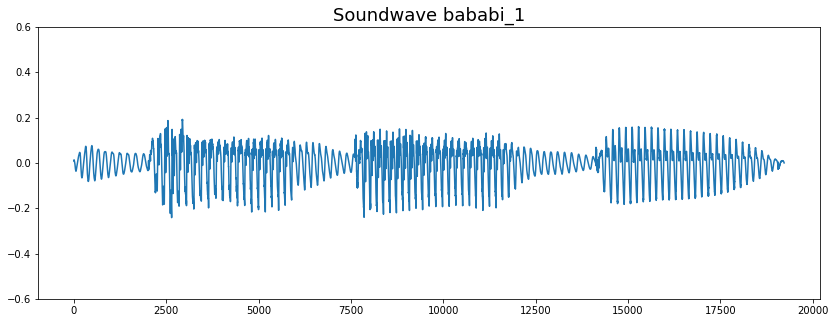
\includegraphics[width=0.5\linewidth]{screenshot017}
					\caption{Sound wave for ``ba ba bi", which should be split up into ``ba", ``ba and ``bi".}
					\label{fig:full sound wave adjusted yaxis}
				\end{subfigure}
				
				\vspace{1em}
				
				
				\begin{subfigure}{\linewidth}
					\centering
					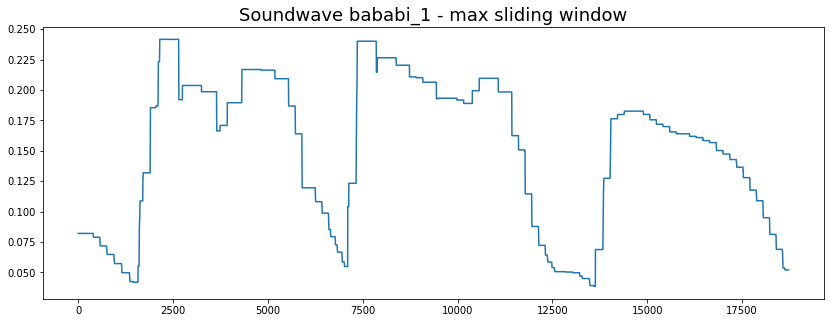
\includegraphics[width=0.5\linewidth]{screenshot012}
					\caption{Resulting speech wave after max pooling. The threshold will be computed using this speech wave.}
					\label{fig:max sliding window}
				\end{subfigure}
				
				\vspace{1em}
				
				\begin{subfigure}{\linewidth}
					\centering
					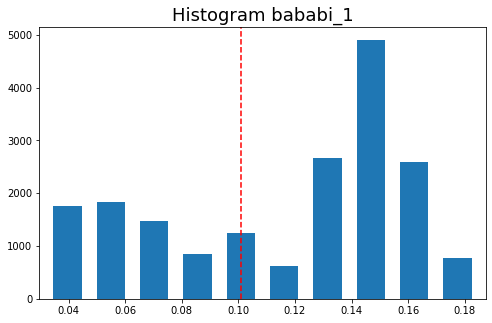
\includegraphics[width=0.3\linewidth]{screenshot018}
					\caption{Threshold obtained using Otsu's algorithm. The red dashed line corresponds to the threshold.}
					\label{fig:histogram}
				\end{subfigure}
				
				\vspace{1em}
				
				\begin{subfigure}{\linewidth}
					\centering
					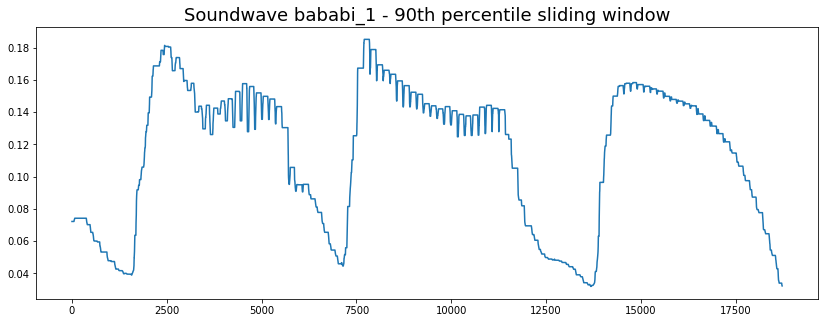
\includegraphics[width=0.5\linewidth]{screenshot013}
					\caption{90'th percentile speech wave (computed using moving window of 0.02 seconds). The threshold is applied to this speech wave. Amplitudes larger than the threshold are considered vowels and smaller values are consonants.}
					\label{fig:90th percentile}
				\end{subfigure}
			
				\vspace{1em}				
				
				\begin{subfigure}{\linewidth}
					\centering
					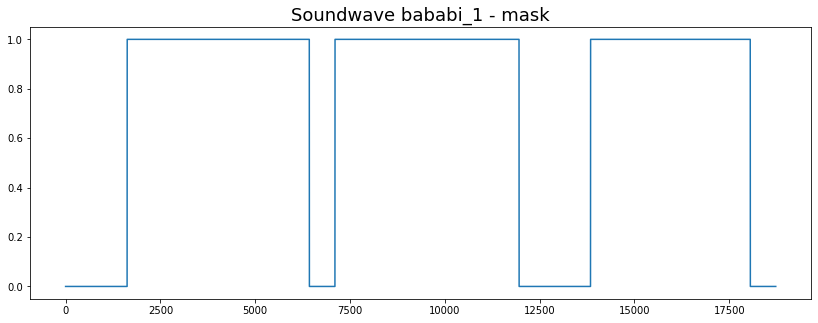
\includegraphics[width=0.5\linewidth]{screenshot014}
					\caption{Obtained mask from applying the threshold. The x coordinates going from one to zero are transition points and mark the end of a syllable. There are three potential points in this image. Since each audio file contains three syllables (and thus a maximum of two transition points), the two \textit{true} points are selected based on their distance from the one-third and two-third x coordinate. In this case, the last transition point will be discarded.}
					\label{fig:mask}
				\end{subfigure}
				
				\vspace{1em}
				
				\begin{subfigure}{\linewidth}
					\centering
					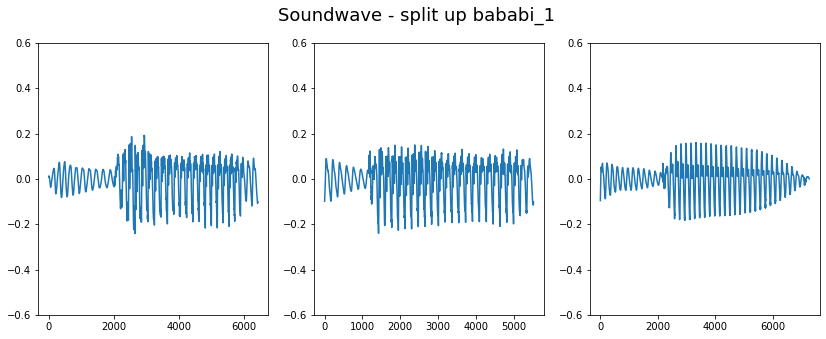
\includegraphics[width=0.5\linewidth]{screenshot016}
					\caption{The three obtained syllables after cutting the speech wave at the two transition points.}
					\label{fig:split up sound wave}
				\end{subfigure}
			\end{minipage}			
		\end{figure}
	



	




%	\section{GIM: Activation visualisations}
%	
%	%these were notes from the decoder from file: eval_autoencoder.py
%	thought for later: its actually weird i was able to play enc as audio as enc is 512 x something
%	so huh? that means that a lot of info is already in first channel? what do other 511 channels then contain?
%	"""
%	Observations:
%	First layer decoded still contains the same sound, but with some added noise (could be because decoder hasn't trained very).
%	However, the encoded first layer, still contains the exact sound as the original sound. It is however downsampled a lot -> from 16khz to ~3khz
%	"""
%	thought for later: its actually weird i was able to play enc as audio as enc is 512 x something
%	so huh? that means that a lot of info is already in first channel? what do other 511 channels then contain?
%	
%	
%	
%	\begin{figure}[h]
%		\centering
%		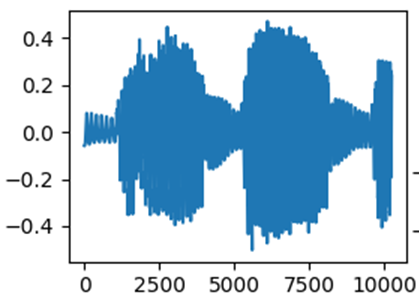
\includegraphics[width=0.7\linewidth]{screenshot007}
%		\caption{"BA-BA-BA" time domain}
%		\label{fig:screenshot007}
%	\end{figure}
%	
%	\begin{figure}[h]
%		\centering
%		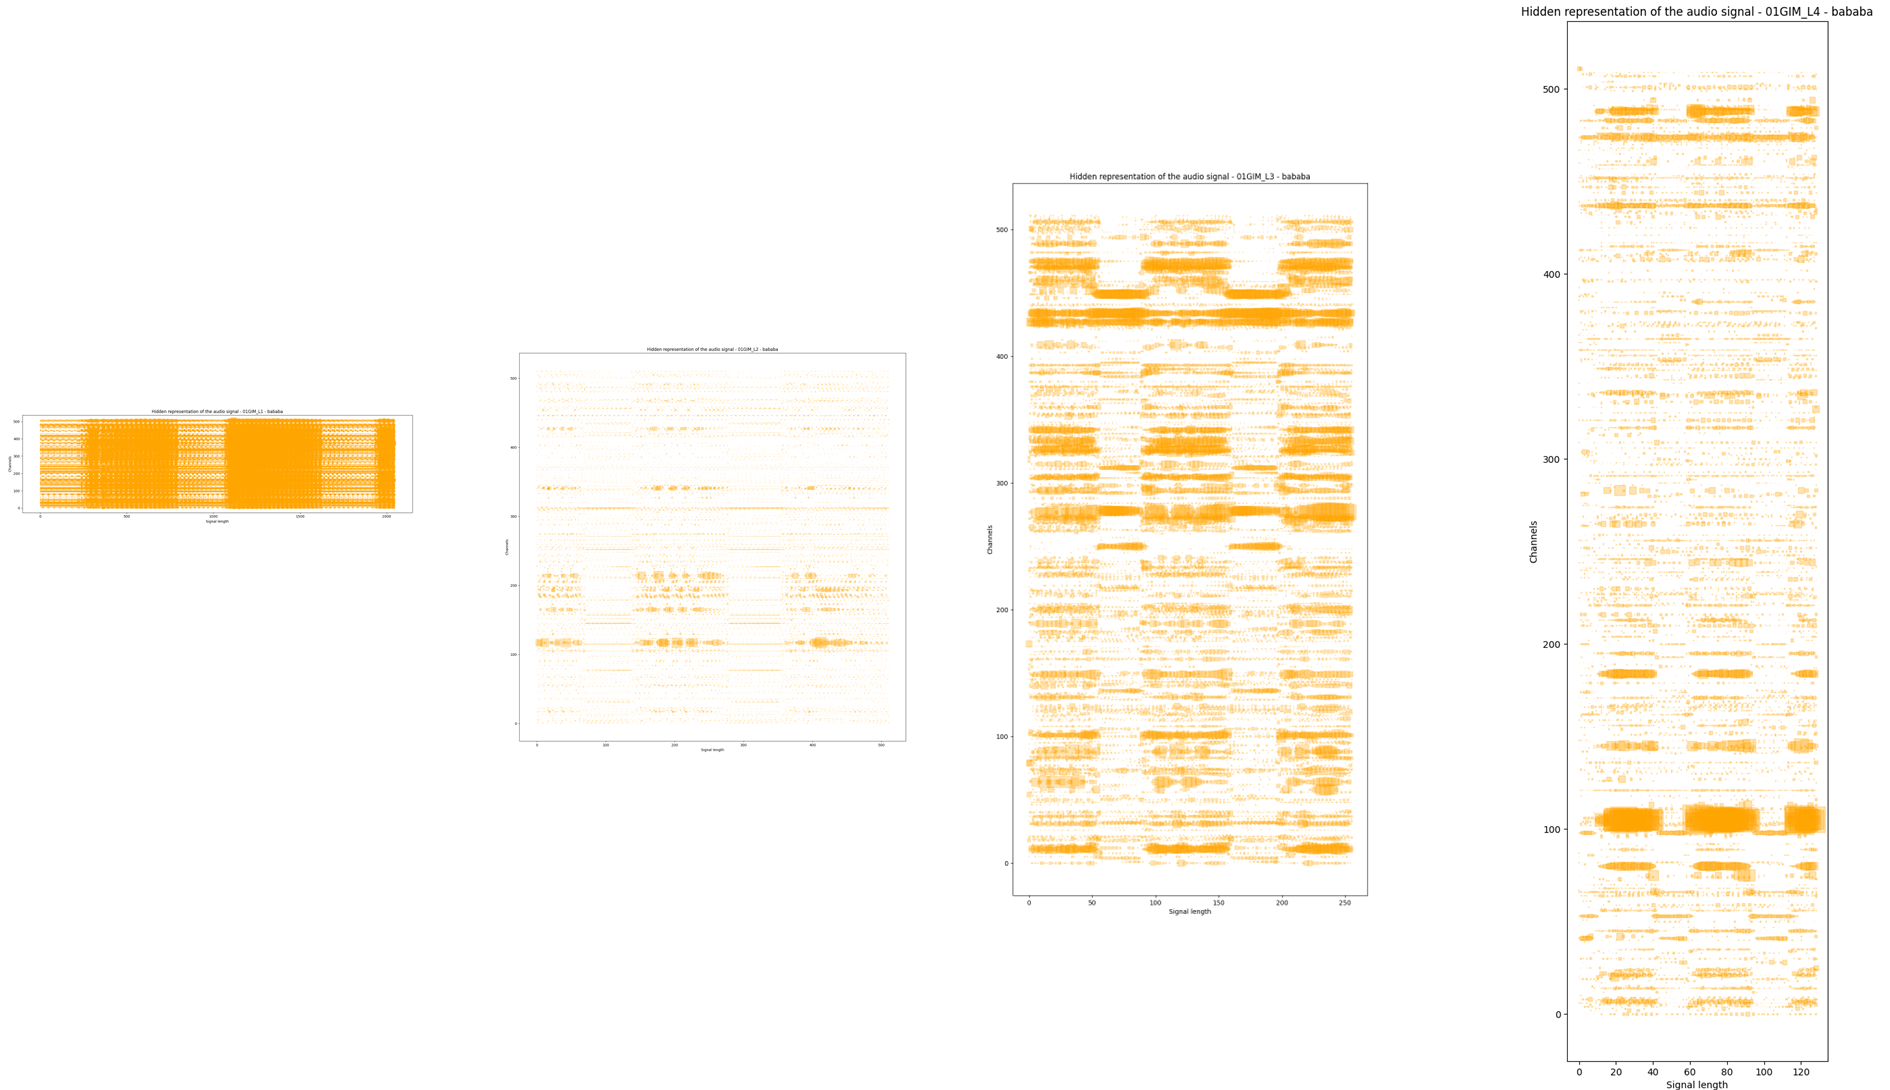
\includegraphics[width=0.7\linewidth]{screenshot006}
%		\caption{Activations of the sound "BA-BA-BA" through GIM}
%		\label{fig:gim latent activations}
%	\end{figure}
%	
%	No batch normalisation, so although channels appear to have larger activations than other channels, size of activation does not really say anything about information. eg activations 0.01 could still contain more information than 3.0 activation.
%	
%	Since the activations from convolutional neural networks, the order is still maintained. Hence, can align activations with original signal.
%	
%	Observations in latent representations:
%	
%	\textit{Layer 1:}
%	The activations of the first decoder still contain a lot of similarity with the original signal, in terms of structure. There is a lot of redundant data within the representation. Eg: the one channel could be replied 
%	
%	Layer 2
%	
%	Layer 3:
%	
%	Layer 4:
%	Still notices multiple channels which have high activations when signal is has high amplitudes and small activations when amplitude is low. 
%	
%	Also activations which are high when volume is low. --> indicates that certain kernel weights are sensitive for \textbf{"klinkers"} and other kernels for \textbf{medeklinkers}. see \ref{fig:screenshot008}.
%	
%	\begin{figure}[h]
%		\centering
%		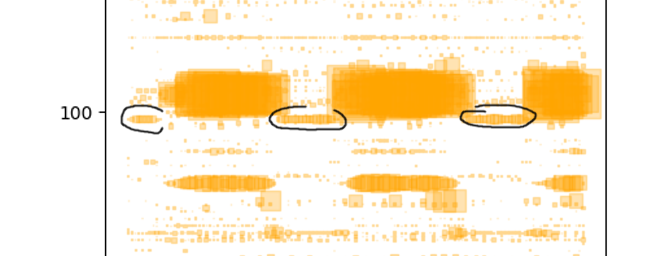
\includegraphics[width=0.7\linewidth]{screenshot008}
%		\caption{zoomed in}
%		\label{fig:screenshot008}
%	\end{figure}
%	
%	
%	Observe that activations happen in clusters/sequences. So it is usually a patch of signal samples that cause high activations. This could for instance indicate that both kernels are sensitive for the \textbf{medeklinker} "b", but sensitive for different features. eg the letter B has spoken sound "buh". so maybe one is sensitive for "b" and other for "uh".
%	
%	Figure \ref{fig:layer4 zoomed in} also nicely shows how different channels have clusters of activations at slightly different times. 
%	
%	\begin{figure}[h]
%		\centering
%		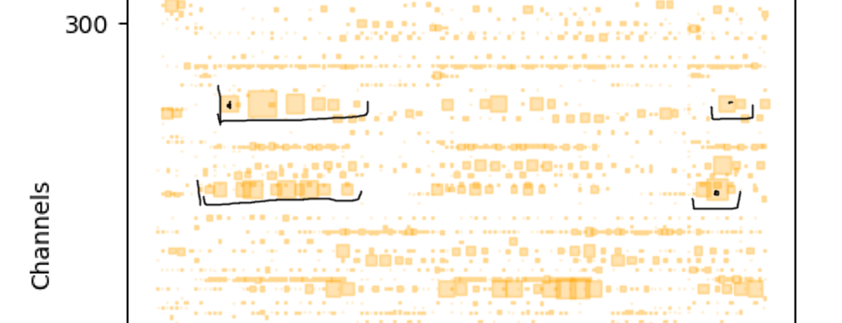
\includegraphics[width=0.7\linewidth]{screenshot010}
%		\caption{Zoomed in}
%		\label{fig:layer4 zoomed in}
%	\end{figure}
	
	

\end{appendices}

\end{document}
